% Options for packages loaded elsewhere
\PassOptionsToPackage{unicode}{hyperref}
\PassOptionsToPackage{hyphens}{url}
\PassOptionsToPackage{dvipsnames,svgnames,x11names}{xcolor}
%
\documentclass[
  11pt,
  a4paper,
]{article}
\usepackage{amsmath,amssymb}
\usepackage{lmodern}
\usepackage{iftex}
\ifPDFTeX
  \usepackage[T1]{fontenc}
  \usepackage[utf8]{inputenc}
  \usepackage{textcomp} % provide euro and other symbols
\else % if luatex or xetex
  \usepackage{unicode-math}
  \defaultfontfeatures{Scale=MatchLowercase}
  \defaultfontfeatures[\rmfamily]{Ligatures=TeX,Scale=1}
\fi
% Use upquote if available, for straight quotes in verbatim environments
\IfFileExists{upquote.sty}{\usepackage{upquote}}{}
\IfFileExists{microtype.sty}{% use microtype if available
  \usepackage[]{microtype}
  \UseMicrotypeSet[protrusion]{basicmath} % disable protrusion for tt fonts
}{}
\makeatletter
\@ifundefined{KOMAClassName}{% if non-KOMA class
  \IfFileExists{parskip.sty}{%
    \usepackage{parskip}
  }{% else
    \setlength{\parindent}{0pt}
    \setlength{\parskip}{6pt plus 2pt minus 1pt}}
}{% if KOMA class
  \KOMAoptions{parskip=half}}
\makeatother
\usepackage{xcolor}
\usepackage[left=3cm,right=3cm,top=2cm,bottom=2cm]{geometry}
\usepackage{color}
\usepackage{fancyvrb}
\newcommand{\VerbBar}{|}
\newcommand{\VERB}{\Verb[commandchars=\\\{\}]}
\DefineVerbatimEnvironment{Highlighting}{Verbatim}{commandchars=\\\{\}}
% Add ',fontsize=\small' for more characters per line
\usepackage{framed}
\definecolor{shadecolor}{RGB}{248,248,248}
\newenvironment{Shaded}{\begin{snugshade}}{\end{snugshade}}
\newcommand{\AlertTok}[1]{\textcolor[rgb]{0.94,0.16,0.16}{#1}}
\newcommand{\AnnotationTok}[1]{\textcolor[rgb]{0.56,0.35,0.01}{\textbf{\textit{#1}}}}
\newcommand{\AttributeTok}[1]{\textcolor[rgb]{0.77,0.63,0.00}{#1}}
\newcommand{\BaseNTok}[1]{\textcolor[rgb]{0.00,0.00,0.81}{#1}}
\newcommand{\BuiltInTok}[1]{#1}
\newcommand{\CharTok}[1]{\textcolor[rgb]{0.31,0.60,0.02}{#1}}
\newcommand{\CommentTok}[1]{\textcolor[rgb]{0.56,0.35,0.01}{\textit{#1}}}
\newcommand{\CommentVarTok}[1]{\textcolor[rgb]{0.56,0.35,0.01}{\textbf{\textit{#1}}}}
\newcommand{\ConstantTok}[1]{\textcolor[rgb]{0.00,0.00,0.00}{#1}}
\newcommand{\ControlFlowTok}[1]{\textcolor[rgb]{0.13,0.29,0.53}{\textbf{#1}}}
\newcommand{\DataTypeTok}[1]{\textcolor[rgb]{0.13,0.29,0.53}{#1}}
\newcommand{\DecValTok}[1]{\textcolor[rgb]{0.00,0.00,0.81}{#1}}
\newcommand{\DocumentationTok}[1]{\textcolor[rgb]{0.56,0.35,0.01}{\textbf{\textit{#1}}}}
\newcommand{\ErrorTok}[1]{\textcolor[rgb]{0.64,0.00,0.00}{\textbf{#1}}}
\newcommand{\ExtensionTok}[1]{#1}
\newcommand{\FloatTok}[1]{\textcolor[rgb]{0.00,0.00,0.81}{#1}}
\newcommand{\FunctionTok}[1]{\textcolor[rgb]{0.00,0.00,0.00}{#1}}
\newcommand{\ImportTok}[1]{#1}
\newcommand{\InformationTok}[1]{\textcolor[rgb]{0.56,0.35,0.01}{\textbf{\textit{#1}}}}
\newcommand{\KeywordTok}[1]{\textcolor[rgb]{0.13,0.29,0.53}{\textbf{#1}}}
\newcommand{\NormalTok}[1]{#1}
\newcommand{\OperatorTok}[1]{\textcolor[rgb]{0.81,0.36,0.00}{\textbf{#1}}}
\newcommand{\OtherTok}[1]{\textcolor[rgb]{0.56,0.35,0.01}{#1}}
\newcommand{\PreprocessorTok}[1]{\textcolor[rgb]{0.56,0.35,0.01}{\textit{#1}}}
\newcommand{\RegionMarkerTok}[1]{#1}
\newcommand{\SpecialCharTok}[1]{\textcolor[rgb]{0.00,0.00,0.00}{#1}}
\newcommand{\SpecialStringTok}[1]{\textcolor[rgb]{0.31,0.60,0.02}{#1}}
\newcommand{\StringTok}[1]{\textcolor[rgb]{0.31,0.60,0.02}{#1}}
\newcommand{\VariableTok}[1]{\textcolor[rgb]{0.00,0.00,0.00}{#1}}
\newcommand{\VerbatimStringTok}[1]{\textcolor[rgb]{0.31,0.60,0.02}{#1}}
\newcommand{\WarningTok}[1]{\textcolor[rgb]{0.56,0.35,0.01}{\textbf{\textit{#1}}}}
\usepackage{graphicx}
\makeatletter
\def\maxwidth{\ifdim\Gin@nat@width>\linewidth\linewidth\else\Gin@nat@width\fi}
\def\maxheight{\ifdim\Gin@nat@height>\textheight\textheight\else\Gin@nat@height\fi}
\makeatother
% Scale images if necessary, so that they will not overflow the page
% margins by default, and it is still possible to overwrite the defaults
% using explicit options in \includegraphics[width, height, ...]{}
\setkeys{Gin}{width=\maxwidth,height=\maxheight,keepaspectratio}
% Set default figure placement to htbp
\makeatletter
\def\fps@figure{htbp}
\makeatother
\setlength{\emergencystretch}{3em} % prevent overfull lines
\providecommand{\tightlist}{%
  \setlength{\itemsep}{0pt}\setlength{\parskip}{0pt}}
\setcounter{secnumdepth}{5}
\usepackage{fvextra}
\usepackage{mathtools}
\usepackage{longtable}
\usepackage{graphicx}
\usepackage{lscape}
% If you use beamer only pass "xcolor=table" option, i.e. \documentclass[xcolor=table]{beamer}
\usepackage[normalem]{ulem}
\useunder{\uline}{\ul}{}
\usepackage{lscape}
\usepackage{longtable}
\renewcommand{\contentsname}{Índice}
\DeclarePairedDelimiter\ceil{\lceil}{\rceil}
\DeclarePairedDelimiter\floor{\lfloor}{\rfloor}
\DefineVerbatimEnvironment{Highlighting}{Verbatim}{breaklines,commandchars=\\\{\}}
\ifLuaTeX
  \usepackage{selnolig}  % disable illegal ligatures
\fi
\IfFileExists{bookmark.sty}{\usepackage{bookmark}}{\usepackage{hyperref}}
\IfFileExists{xurl.sty}{\usepackage{xurl}}{} % add URL line breaks if available
\urlstyle{same} % disable monospaced font for URLs
\hypersetup{
  colorlinks=true,
  linkcolor={Maroon},
  filecolor={Maroon},
  citecolor={Blue},
  urlcolor={blue},
  pdfcreator={LaTeX via pandoc}}

\author{}
\date{\vspace{-2.5em}}

\begin{document}

%\begin{titlepage}

\graphicspath{ {images/} }

\begin{center}
\centering
	
\includegraphics[width=1.5\textwidth]{uc3m}\par\vspace{1cm}
{\scshape\LARGE Universidad Carlos III de Madrid \par}
	\vspace{1cm}
	{\scshape\Large Aprendizaje Automático, Grado en Estadística y Empresa \par}
	\vspace{1.5cm}
	{\huge\bfseries Práctica I: KNN y Árboles de clasificación \par}
	\vspace{2cm}
	{\Large\itshape Marcos Álvarez Martín \\ Fabio Scielzo Ortiz \par}
	\date{3 de Marzo de 2022}
	\vfill
	\vfill
\end{center}
% \end{titlepage}

\newpage
\tableofcontents
\newpage

\begin{Shaded}
\begin{Highlighting}[]
\ImportTok{import}\NormalTok{ pandas }\ImportTok{as}\NormalTok{ pd}
\end{Highlighting}
\end{Shaded}

\begin{Shaded}
\begin{Highlighting}[]
\NormalTok{df\_Fake }\OperatorTok{=}\NormalTok{ pd.read\_csv(}\StringTok{\textquotesingle{}Fake.csv\textquotesingle{}}\NormalTok{)}
\NormalTok{df\_True }\OperatorTok{=}\NormalTok{ pd.read\_csv(}\StringTok{\textquotesingle{}True.csv\textquotesingle{}}\NormalTok{)}
\end{Highlighting}
\end{Shaded}

\begin{Shaded}
\begin{Highlighting}[]
\NormalTok{df\_Fake[}\StringTok{\textquotesingle{}Fake\textquotesingle{}}\NormalTok{] }\OperatorTok{=} \DecValTok{1}
\NormalTok{df\_True[}\StringTok{\textquotesingle{}Fake\textquotesingle{}}\NormalTok{] }\OperatorTok{=} \DecValTok{0}
\end{Highlighting}
\end{Shaded}

\begin{Shaded}
\begin{Highlighting}[]
\NormalTok{Fake\_News\_Data }\OperatorTok{=}\NormalTok{ pd.concat([df\_Fake, df\_True])}
\end{Highlighting}
\end{Shaded}

\begin{Shaded}
\begin{Highlighting}[]
\NormalTok{Fake\_News\_Data }\OperatorTok{=}\NormalTok{ Fake\_News\_Data.loc[: , [}\StringTok{\textquotesingle{}Fake\textquotesingle{}}\NormalTok{, }\StringTok{\textquotesingle{}title\textquotesingle{}}\NormalTok{, }\StringTok{\textquotesingle{}text\textquotesingle{}}\NormalTok{, }\StringTok{\textquotesingle{}date\textquotesingle{}}\NormalTok{] ]}
\end{Highlighting}
\end{Shaded}

\begin{Shaded}
\begin{Highlighting}[]
\NormalTok{Fake\_News\_Data.index }\OperatorTok{=} \BuiltInTok{range}\NormalTok{(}\DecValTok{0}\NormalTok{ , }\BuiltInTok{len}\NormalTok{(Fake\_News\_Data))}
\end{Highlighting}
\end{Shaded}

Fake = 1 --\textgreater{} yes

Fake = 0 --\textgreater{} no

\begin{Shaded}
\begin{Highlighting}[]
\NormalTok{Fake\_News\_Data.dtypes}
\end{Highlighting}
\end{Shaded}

\begin{verbatim}
Fake      int64
title    object
text     object
date     object
dtype: object
\end{verbatim}

\begin{Shaded}
\begin{Highlighting}[]
\NormalTok{Fake\_News\_Data[}\StringTok{\textquotesingle{}Fake\textquotesingle{}}\NormalTok{] }\OperatorTok{=}\NormalTok{ Fake\_News\_Data[}\StringTok{\textquotesingle{}Fake\textquotesingle{}}\NormalTok{].astype(}\StringTok{\textquotesingle{}object\textquotesingle{}}\NormalTok{)}
\end{Highlighting}
\end{Shaded}

\begin{Shaded}
\begin{Highlighting}[]
\NormalTok{Fake\_News\_Data.describe(include}\OperatorTok{=}\StringTok{\textquotesingle{}all\textquotesingle{}}\NormalTok{)}
\end{Highlighting}
\end{Shaded}

Fake

title

text

date

count

44898

44898

44898

44898

unique

2

38729

38646

2397

top

1

Factbox: Trump fills top jobs for his administ\ldots{}

December 20, 2017

freq

23481

14

627

182

\begin{Shaded}
\begin{Highlighting}[]
\NormalTok{Fake\_News\_Data.isnull().}\BuiltInTok{sum}\NormalTok{()}
\end{Highlighting}
\end{Shaded}

\begin{verbatim}
Fake     0
title    0
text     0
date     0
dtype: int64
\end{verbatim}

\begin{Shaded}
\begin{Highlighting}[]
\ImportTok{import}\NormalTok{ numpy }\ImportTok{as}\NormalTok{ np}

\ImportTok{import}\NormalTok{ seaborn }\ImportTok{as}\NormalTok{ sns}
\ImportTok{import}\NormalTok{ matplotlib }\ImportTok{as}\NormalTok{ mpl}
\ImportTok{import}\NormalTok{ matplotlib.pyplot }\ImportTok{as}\NormalTok{ plt}

\NormalTok{sns.}\BuiltInTok{set}\NormalTok{(rc}\OperatorTok{=}\NormalTok{\{}\StringTok{\textquotesingle{}figure.figsize\textquotesingle{}}\NormalTok{:(}\DecValTok{8}\NormalTok{,}\DecValTok{8}\NormalTok{)\})}
\end{Highlighting}
\end{Shaded}

\begin{Shaded}
\begin{Highlighting}[]
\NormalTok{prop\_Fake\_yes }\OperatorTok{=} \BuiltInTok{len}\NormalTok{( Fake\_News\_Data.loc[ Fake\_News\_Data[}\StringTok{\textquotesingle{}Fake\textquotesingle{}}\NormalTok{]}\OperatorTok{==} \DecValTok{1}\NormalTok{ , :] ) }\OperatorTok{/} \BuiltInTok{len}\NormalTok{(Fake\_News\_Data)}

\NormalTok{prop\_Fake\_no }\OperatorTok{=} \BuiltInTok{len}\NormalTok{( Fake\_News\_Data.loc[ Fake\_News\_Data[}\StringTok{\textquotesingle{}Fake\textquotesingle{}}\NormalTok{]}\OperatorTok{==} \DecValTok{0}\NormalTok{ , :] ) }\OperatorTok{/} \BuiltInTok{len}\NormalTok{(Fake\_News\_Data)}
\end{Highlighting}
\end{Shaded}

\begin{Shaded}
\begin{Highlighting}[]
\NormalTok{Fake\_News\_Data[}\StringTok{\textquotesingle{}proportion\_Fakes\textquotesingle{}}\NormalTok{] }\OperatorTok{=} \DecValTok{0}


\ControlFlowTok{for}\NormalTok{ i }\KeywordTok{in} \BuiltInTok{range}\NormalTok{(}\DecValTok{0}\NormalTok{, }\BuiltInTok{len}\NormalTok{(Fake\_News\_Data)):}

    \ControlFlowTok{if}\NormalTok{ Fake\_News\_Data[}\StringTok{\textquotesingle{}Fake\textquotesingle{}}\NormalTok{][i] }\OperatorTok{==} \DecValTok{1}\NormalTok{ :}

\NormalTok{        Fake\_News\_Data[}\StringTok{\textquotesingle{}proportion\_Fakes\textquotesingle{}}\NormalTok{][i] }\OperatorTok{=}\NormalTok{ prop\_Fake\_yes}

    \ControlFlowTok{else}\NormalTok{ :}

\NormalTok{        Fake\_News\_Data[}\StringTok{\textquotesingle{}proportion\_Fakes\textquotesingle{}}\NormalTok{][i] }\OperatorTok{=}\NormalTok{ prop\_Fake\_no}
\end{Highlighting}
\end{Shaded}

\begin{verbatim}
C:\Users\Usuario\AppData\Local\Temp\ipykernel_19644\2699169446.py:8: SettingWithCopyWarning: 
A value is trying to be set on a copy of a slice from a DataFrame

See the caveats in the documentation: https://pandas.pydata.org/pandas-docs/stable/user_guide/indexing.html#returning-a-view-versus-a-copy
  Fake_News_Data['proportion_Fakes'][i] = prop_Fake_yes
\end{verbatim}

\begin{Shaded}
\begin{Highlighting}[]
\NormalTok{p1 }\OperatorTok{=}\NormalTok{ sns.barplot(x}\OperatorTok{=}\StringTok{\textquotesingle{}Fake\textquotesingle{}}\NormalTok{, y}\OperatorTok{=}\StringTok{\textquotesingle{}proportion\_Fakes\textquotesingle{}}\NormalTok{, data}\OperatorTok{=}\NormalTok{Fake\_News\_Data, palette}\OperatorTok{=}\StringTok{"Spectral"}\NormalTok{) }
\NormalTok{p1.set\_yticks( np.arange(}\DecValTok{0}\NormalTok{, }\FloatTok{0.85}\NormalTok{, }\FloatTok{0.1}\NormalTok{)  )}
\NormalTok{p1.set\_xticklabels([}\StringTok{\textquotesingle{}No\textquotesingle{}}\NormalTok{, }\StringTok{\textquotesingle{}Yes\textquotesingle{}}\NormalTok{])}
\NormalTok{p1.axes.}\BuiltInTok{set}\NormalTok{(xlabel}\OperatorTok{=}\StringTok{\textquotesingle{}Fakes\textquotesingle{}}\NormalTok{, ylabel}\OperatorTok{=}\StringTok{\textquotesingle{}proportion\textquotesingle{}}\NormalTok{)}
\end{Highlighting}
\end{Shaded}

\begin{verbatim}
[Text(0.5, 0, 'Fakes'), Text(0, 0.5, 'proportion')]
\end{verbatim}

\begin{figure}
\centering
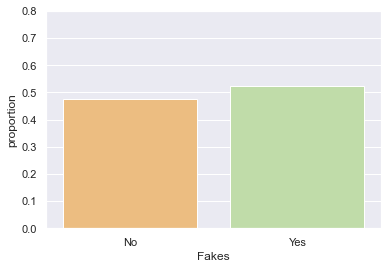
\includegraphics{output_15_1.png}
\caption{png}
\end{figure}

\begin{Shaded}
\begin{Highlighting}[]
\NormalTok{[prop\_Fake\_no , prop\_Fake\_yes]}
\end{Highlighting}
\end{Shaded}

\begin{verbatim}
[0.47701456635039424, 0.5229854336496058]
\end{verbatim}

\begin{Shaded}
\begin{Highlighting}[]
\NormalTok{[prop\_Fake\_no}\OperatorTok{*}\BuiltInTok{len}\NormalTok{(Fake\_News\_Data) , prop\_Fake\_yes}\OperatorTok{*}\BuiltInTok{len}\NormalTok{(Fake\_News\_Data)]}
\end{Highlighting}
\end{Shaded}

\begin{verbatim}
[21417.0, 23481.0]
\end{verbatim}

\begin{Shaded}
\begin{Highlighting}[]
\NormalTok{Fake\_News\_Data }\OperatorTok{=}\NormalTok{ Fake\_News\_Data.loc[ : , Fake\_News\_Data.columns }\OperatorTok{!=} \StringTok{\textquotesingle{}proportion\_Fakes\textquotesingle{}}\NormalTok{]}
\end{Highlighting}
\end{Shaded}

\begin{Shaded}
\begin{Highlighting}[]
\NormalTok{Fake\_News\_Data[}\StringTok{\textquotesingle{}word\_count\textquotesingle{}}\NormalTok{] }\OperatorTok{=}\NormalTok{ Fake\_News\_Data[}\StringTok{\textquotesingle{}text\textquotesingle{}}\NormalTok{].}\BuiltInTok{str}\NormalTok{.split().}\BuiltInTok{str}\NormalTok{.}\BuiltInTok{len}\NormalTok{()}
\end{Highlighting}
\end{Shaded}

\begin{Shaded}
\begin{Highlighting}[]
\NormalTok{Fake\_News\_Data}
\end{Highlighting}
\end{Shaded}

Fake

title

text

date

word\_count

0

1

Donald Trump Sends Out Embarrassing New Year'\ldots{}

Donald Trump just couldn t wish all Americans \ldots{}

December 31, 2017

495

1

1

Drunk Bragging Trump Staffer Started Russian \ldots{}

House Intelligence Committee Chairman Devin Nu\ldots{}

December 31, 2017

305

2

1

Sheriff David Clarke Becomes An Internet Joke\ldots{}

On Friday, it was revealed that former Milwauk\ldots{}

December 30, 2017

580

3

1

Trump Is So Obsessed He Even Has Obama's Name\ldots{}

On Christmas day, Donald Trump announced that \ldots{}

December 29, 2017

444

4

1

Pope Francis Just Called Out Donald Trump Dur\ldots{}

Pope Francis used his annual Christmas Day mes\ldots{}

December 25, 2017

420

\ldots{}

\ldots{}

\ldots{}

\ldots{}

\ldots{}

\ldots{}

44893

0

`Fully committed' NATO backs new U.S. approach\ldots{}

BRUSSELS (Reuters) - NATO allies on Tuesday we\ldots{}

August 22, 2017

466

44894

0

LexisNexis withdrew two products from Chinese \ldots{}

LONDON (Reuters) - LexisNexis, a provider of l\ldots{}

August 22, 2017

125

44895

0

Minsk cultural hub becomes haven from authorities

MINSK (Reuters) - In the shadow of disused Sov\ldots{}

August 22, 2017

320

44896

0

Vatican upbeat on possibility of Pope Francis \ldots{}

MOSCOW (Reuters) - Vatican Secretary of State \ldots{}

August 22, 2017

205

44897

0

Indonesia to buy \$1.14 billion worth of Russia\ldots{}

JAKARTA (Reuters) - Indonesia will buy 11 Sukh\ldots{}

August 22, 2017

210

44898 rows × 5 columns

\begin{Shaded}
\begin{Highlighting}[]
\NormalTok{Fake\_News\_Data.groupby(}\StringTok{\textquotesingle{}Fake\textquotesingle{}}\NormalTok{)[}\StringTok{\textquotesingle{}word\_count\textquotesingle{}}\NormalTok{].mean()}
\end{Highlighting}
\end{Shaded}

\begin{verbatim}
Fake
0    385.640099
1    423.197905
Name: word_count, dtype: float64
\end{verbatim}

\begin{Shaded}
\begin{Highlighting}[]
\KeywordTok{def}\NormalTok{ limpiar\_tokenizar(texto):}

    \ImportTok{import}\NormalTok{ re}
    
    \CommentTok{\textquotesingle{}\textquotesingle{}\textquotesingle{}}
\CommentTok{    Esta función limpia y tokeniza el texto en palabras individuales.}
\CommentTok{    El orden en el que se va limpiando el texto no es arbitrario.}
\CommentTok{    El listado de signos de puntuación se ha obtenido de: print(string.punctuation)}
\CommentTok{    y re.escape(string.punctuation)}
\CommentTok{    \textquotesingle{}\textquotesingle{}\textquotesingle{}}
    
    \CommentTok{\# Se convierte todo el texto a minúsculas}

\NormalTok{    nuevo\_texto }\OperatorTok{=}\NormalTok{ texto.lower()}
    
    \CommentTok{\# Eliminacion de paginas web (palabras que empiezan por "http")}
    
\NormalTok{    nuevo\_texto }\OperatorTok{=}\NormalTok{ re.sub(}\StringTok{\textquotesingle{}http\textbackslash{}S+\textquotesingle{}}\NormalTok{, }\StringTok{\textquotesingle{} \textquotesingle{}}\NormalTok{, nuevo\_texto)}
    
    \CommentTok{\# Eliminacion de signos de puntuación}
    
\NormalTok{    regex }\OperatorTok{=} \StringTok{\textquotesingle{}[}\CharTok{\textbackslash{}\textbackslash{}}\StringTok{!}\CharTok{\textbackslash{}\textbackslash{}}\StringTok{"}\CharTok{\textbackslash{}\textbackslash{}}\StringTok{\#}\CharTok{\textbackslash{}\textbackslash{}}\StringTok{$}\CharTok{\textbackslash{}\textbackslash{}}\StringTok{\%}\CharTok{\textbackslash{}\textbackslash{}}\StringTok{\&}\CharTok{\textbackslash{}\textbackslash{}\textbackslash{}\textquotesingle{}\textbackslash{}\textbackslash{}}\StringTok{(}\CharTok{\textbackslash{}\textbackslash{}}\StringTok{)}\CharTok{\textbackslash{}\textbackslash{}}\StringTok{*}\CharTok{\textbackslash{}\textbackslash{}}\StringTok{+}\CharTok{\textbackslash{}\textbackslash{}}\StringTok{,}\CharTok{\textbackslash{}\textbackslash{}}\StringTok{{-}}\CharTok{\textbackslash{}\textbackslash{}}\StringTok{.}\CharTok{\textbackslash{}\textbackslash{}}\StringTok{/}\CharTok{\textbackslash{}\textbackslash{}}\StringTok{:}\CharTok{\textbackslash{}\textbackslash{}}\StringTok{;}\CharTok{\textbackslash{}\textbackslash{}}\StringTok{\textless{}}\CharTok{\textbackslash{}\textbackslash{}}\StringTok{=}\CharTok{\textbackslash{}\textbackslash{}}\StringTok{\textgreater{}}\CharTok{\textbackslash{}\textbackslash{}}\StringTok{?}\CharTok{\textbackslash{}\textbackslash{}}\StringTok{@}\CharTok{\textbackslash{}\textbackslash{}}\StringTok{[}\CharTok{\textbackslash{}\textbackslash{}\textbackslash{}\textbackslash{}\textbackslash{}\textbackslash{}}\StringTok{]}\CharTok{\textbackslash{}\textbackslash{}}\StringTok{\^{}\_}\CharTok{\textbackslash{}\textbackslash{}}\StringTok{\textasciigrave{}}\CharTok{\textbackslash{}\textbackslash{}}\StringTok{\{}\CharTok{\textbackslash{}\textbackslash{}}\StringTok{|}\CharTok{\textbackslash{}\textbackslash{}}\StringTok{\}}\CharTok{\textbackslash{}\textbackslash{}}\StringTok{\textasciitilde{}]\textquotesingle{}}
    
\NormalTok{    nuevo\_texto }\OperatorTok{=}\NormalTok{ re.sub(regex , }\StringTok{\textquotesingle{} \textquotesingle{}}\NormalTok{, nuevo\_texto)}
    
    \CommentTok{\# Eliminacion de numeros}
    
\NormalTok{    nuevo\_texto }\OperatorTok{=}\NormalTok{ re.sub(}\StringTok{"\textbackslash{}d+"}\NormalTok{, }\StringTok{\textquotesingle{} \textquotesingle{}}\NormalTok{, nuevo\_texto)}
    
    \CommentTok{\# Eliminacion de espacios en blanco multiples}
    
\NormalTok{    nuevo\_texto }\OperatorTok{=}\NormalTok{ re.sub(}\StringTok{"}\CharTok{\textbackslash{}\textbackslash{}}\StringTok{s+"}\NormalTok{, }\StringTok{\textquotesingle{} \textquotesingle{}}\NormalTok{, nuevo\_texto)}
    
    \CommentTok{\# Tokenizacion por palabras individuales}
    
\NormalTok{    nuevo\_texto }\OperatorTok{=}\NormalTok{ nuevo\_texto.split(sep }\OperatorTok{=} \StringTok{\textquotesingle{} \textquotesingle{}}\NormalTok{)}
    
    \CommentTok{\# Eliminacion de tokens con una longitud \textless{}= 1}
    
\NormalTok{    nuevo\_texto }\OperatorTok{=}\NormalTok{ [token }\ControlFlowTok{for}\NormalTok{ token }\KeywordTok{in}\NormalTok{ nuevo\_texto }\ControlFlowTok{if} \BuiltInTok{len}\NormalTok{(token) }\OperatorTok{\textgreater{}=}  \DecValTok{2}\NormalTok{]}
    
    \ControlFlowTok{return}\NormalTok{(nuevo\_texto)}
\end{Highlighting}
\end{Shaded}

\begin{Shaded}
\begin{Highlighting}[]

\NormalTok{test }\OperatorTok{=} \StringTok{"Esto es 1 ejemplo de l\textquotesingle{}limpieza de6 TEXTO  https://t.co/rnHPgyhx4Z @cienciadedatos \#textmining"}

\BuiltInTok{print}\NormalTok{(limpiar\_tokenizar(texto}\OperatorTok{=}\NormalTok{test))}
\end{Highlighting}
\end{Shaded}

\begin{verbatim}
['esto', 'es', 'ejemplo', 'de', 'limpieza', 'de', 'texto', 'cienciadedatos', 'textmining']
\end{verbatim}

\begin{Shaded}
\begin{Highlighting}[]
\NormalTok{Fake\_News\_Data[}\StringTok{\textquotesingle{}text\textquotesingle{}}\NormalTok{][}\DecValTok{0}\NormalTok{]}
\end{Highlighting}
\end{Shaded}

\begin{verbatim}
'Donald Trump just couldn t wish all Americans a Happy New Year and leave it at that. Instead, he had to give a shout out to his enemies, haters and  the very dishonest fake news media.  The former reality show star had just one job to do and he couldn t do it. As our Country rapidly grows stronger and smarter, I want to wish all of my friends, supporters, enemies, haters, and even the very dishonest Fake News Media, a Happy and Healthy New Year,  President Angry Pants tweeted.  2018 will be a great year for America! As our Country rapidly grows stronger and smarter, I want to wish all of my friends, supporters, enemies, haters, and even the very dishonest Fake News Media, a Happy and Healthy New Year. 2018 will be a great year for America!  Donald J. Trump (@realDonaldTrump) December 31, 2017Trump s tweet went down about as welll as you d expect.What kind of president sends a New Year s greeting like this despicable, petty, infantile gibberish? Only Trump! His lack of decency won t even allow him to rise above the gutter long enough to wish the American citizens a happy new year!  Bishop Talbert Swan (@TalbertSwan) December 31, 2017no one likes you  Calvin (@calvinstowell) December 31, 2017Your impeachment would make 2018 a great year for America, but I ll also accept regaining control of Congress.  Miranda Yaver (@mirandayaver) December 31, 2017Do you hear yourself talk? When you have to include that many people that hate you you have to wonder? Why do the they all hate me?  Alan Sandoval (@AlanSandoval13) December 31, 2017Who uses the word Haters in a New Years wish??  Marlene (@marlene399) December 31, 2017You can t just say happy new year?  Koren pollitt (@Korencarpenter) December 31, 2017Here s Trump s New Year s Eve tweet from 2016.Happy New Year to all, including to my many enemies and those who have fought me and lost so badly they just don t know what to do. Love!  Donald J. Trump (@realDonaldTrump) December 31, 2016This is nothing new for Trump. He s been doing this for years.Trump has directed messages to his  enemies  and  haters  for New Year s, Easter, Thanksgiving, and the anniversary of 9/11. pic.twitter.com/4FPAe2KypA  Daniel Dale (@ddale8) December 31, 2017Trump s holiday tweets are clearly not presidential.How long did he work at Hallmark before becoming President?  Steven Goodine (@SGoodine) December 31, 2017He s always been like this . . . the only difference is that in the last few years, his filter has been breaking down.  Roy Schulze (@thbthttt) December 31, 2017Who, apart from a teenager uses the term haters?  Wendy (@WendyWhistles) December 31, 2017he s a fucking 5 year old  Who Knows (@rainyday80) December 31, 2017So, to all the people who voted for this a hole thinking he would change once he got into power, you were wrong! 70-year-old men don t change and now he s a year older.Photo by Andrew Burton/Getty Images.'
\end{verbatim}

\begin{Shaded}
\begin{Highlighting}[]
\BuiltInTok{print}\NormalTok{(limpiar\_tokenizar(texto}\OperatorTok{=}\NormalTok{Fake\_News\_Data[}\StringTok{\textquotesingle{}text\textquotesingle{}}\NormalTok{][}\DecValTok{0}\NormalTok{]))}
\end{Highlighting}
\end{Shaded}

\begin{verbatim}
['donald', 'trump', 'just', 'couldn', 'wish', 'all', 'americans', 'happy', 'new', 'year', 'and', 'leave', 'it', 'at', 'that', 'instead', 'he', 'had', 'to', 'give', 'shout', 'out', 'to', 'his', 'enemies', 'haters', 'and', 'the', 'very', 'dishonest', 'fake', 'news', 'media', 'the', 'former', 'reality', 'show', 'star', 'had', 'just', 'one', 'job', 'to', 'do', 'and', 'he', 'couldn', 'do', 'it', 'as', 'our', 'country', 'rapidly', 'grows', 'stronger', 'and', 'smarter', 'want', 'to', 'wish', 'all', 'of', 'my', 'friends', 'supporters', 'enemies', 'haters', 'and', 'even', 'the', 'very', 'dishonest', 'fake', 'news', 'media', 'happy', 'and', 'healthy', 'new', 'year', 'president', 'angry', 'pants', 'tweeted', 'will', 'be', 'great', 'year', 'for', 'america', 'as', 'our', 'country', 'rapidly', 'grows', 'stronger', 'and', 'smarter', 'want', 'to', 'wish', 'all', 'of', 'my', 'friends', 'supporters', 'enemies', 'haters', 'and', 'even', 'the', 'very', 'dishonest', 'fake', 'news', 'media', 'happy', 'and', 'healthy', 'new', 'year', 'will', 'be', 'great', 'year', 'for', 'america', 'donald', 'trump', 'realdonaldtrump', 'december', 'trump', 'tweet', 'went', 'down', 'about', 'as', 'welll', 'as', 'you', 'expect', 'what', 'kind', 'of', 'president', 'sends', 'new', 'year', 'greeting', 'like', 'this', 'despicable', 'petty', 'infantile', 'gibberish', 'only', 'trump', 'his', 'lack', 'of', 'decency', 'won', 'even', 'allow', 'him', 'to', 'rise', 'above', 'the', 'gutter', 'long', 'enough', 'to', 'wish', 'the', 'american', 'citizens', 'happy', 'new', 'year', 'bishop', 'talbert', 'swan', 'talbertswan', 'december', 'no', 'one', 'likes', 'you', 'calvin', 'calvinstowell', 'december', 'your', 'impeachment', 'would', 'make', 'great', 'year', 'for', 'america', 'but', 'll', 'also', 'accept', 'regaining', 'control', 'of', 'congress', 'miranda', 'yaver', 'mirandayaver', 'december', 'do', 'you', 'hear', 'yourself', 'talk', 'when', 'you', 'have', 'to', 'include', 'that', 'many', 'people', 'that', 'hate', 'you', 'you', 'have', 'to', 'wonder', 'why', 'do', 'the', 'they', 'all', 'hate', 'me', 'alan', 'sandoval', 'alansandoval', 'december', 'who', 'uses', 'the', 'word', 'haters', 'in', 'new', 'years', 'wish', 'marlene', 'marlene', 'december', 'you', 'can', 'just', 'say', 'happy', 'new', 'year', 'koren', 'pollitt', 'korencarpenter', 'december', 'here', 'trump', 'new', 'year', 'eve', 'tweet', 'from', 'happy', 'new', 'year', 'to', 'all', 'including', 'to', 'my', 'many', 'enemies', 'and', 'those', 'who', 'have', 'fought', 'me', 'and', 'lost', 'so', 'badly', 'they', 'just', 'don', 'know', 'what', 'to', 'do', 'love', 'donald', 'trump', 'realdonaldtrump', 'december', 'this', 'is', 'nothing', 'new', 'for', 'trump', 'he', 'been', 'doing', 'this', 'for', 'years', 'trump', 'has', 'directed', 'messages', 'to', 'his', 'enemies', 'and', 'haters', 'for', 'new', 'year', 'easter', 'thanksgiving', 'and', 'the', 'anniversary', 'of', 'pic', 'twitter', 'com', 'fpae', 'kypa', 'daniel', 'dale', 'ddale', 'december', 'trump', 'holiday', 'tweets', 'are', 'clearly', 'not', 'presidential', 'how', 'long', 'did', 'he', 'work', 'at', 'hallmark', 'before', 'becoming', 'president', 'steven', 'goodine', 'sgoodine', 'december', 'he', 'always', 'been', 'like', 'this', 'the', 'only', 'difference', 'is', 'that', 'in', 'the', 'last', 'few', 'years', 'his', 'filter', 'has', 'been', 'breaking', 'down', 'roy', 'schulze', 'thbthttt', 'december', 'who', 'apart', 'from', 'teenager', 'uses', 'the', 'term', 'haters', 'wendy', 'wendywhistles', 'december', 'he', 'fucking', 'year', 'old', 'who', 'knows', 'rainyday', 'december', 'so', 'to', 'all', 'the', 'people', 'who', 'voted', 'for', 'this', 'hole', 'thinking', 'he', 'would', 'change', 'once', 'he', 'got', 'into', 'power', 'you', 'were', 'wrong', 'year', 'old', 'men', 'don', 'change', 'and', 'now', 'he', 'year', 'older', 'photo', 'by', 'andrew', 'burton', 'getty', 'images']
\end{verbatim}

\begin{Shaded}
\begin{Highlighting}[]
\NormalTok{Fake\_News\_Data[}\StringTok{\textquotesingle{}text\_tokenizado\textquotesingle{}}\NormalTok{] }\OperatorTok{=}\NormalTok{ Fake\_News\_Data[}\StringTok{\textquotesingle{}text\textquotesingle{}}\NormalTok{].}\BuiltInTok{apply}\NormalTok{( limpiar\_tokenizar )}
\end{Highlighting}
\end{Shaded}

\begin{Shaded}
\begin{Highlighting}[]
\NormalTok{Fake\_News\_Data[}\StringTok{\textquotesingle{}id\_text\textquotesingle{}}\NormalTok{] }\OperatorTok{=} \BuiltInTok{range}\NormalTok{(}\DecValTok{0}\NormalTok{, }\BuiltInTok{len}\NormalTok{(Fake\_News\_Data))}
\end{Highlighting}
\end{Shaded}

\begin{Shaded}
\begin{Highlighting}[]
\NormalTok{Fake\_News\_Data}
\end{Highlighting}
\end{Shaded}

Fake

title

text

date

word\_count

text\_tokenizado

id\_text

0

1

Donald Trump Sends Out Embarrassing New Year'\ldots{}

Donald Trump just couldn t wish all Americans \ldots{}

December 31, 2017

495

{[}donald, trump, just, couldn, wish, all, ameri\ldots{}

0

1

1

Drunk Bragging Trump Staffer Started Russian \ldots{}

House Intelligence Committee Chairman Devin Nu\ldots{}

December 31, 2017

305

{[}house, intelligence, committee, chairman, dev\ldots{}

1

2

1

Sheriff David Clarke Becomes An Internet Joke\ldots{}

On Friday, it was revealed that former Milwauk\ldots{}

December 30, 2017

580

{[}on, friday, it, was, revealed, that, former, \ldots{}

2

3

1

Trump Is So Obsessed He Even Has Obama's Name\ldots{}

On Christmas day, Donald Trump announced that \ldots{}

December 29, 2017

444

{[}on, christmas, day, donald, trump, announced,\ldots{}

3

4

1

Pope Francis Just Called Out Donald Trump Dur\ldots{}

Pope Francis used his annual Christmas Day mes\ldots{}

December 25, 2017

420

{[}pope, francis, used, his, annual, christmas, \ldots{}

4

\ldots{}

\ldots{}

\ldots{}

\ldots{}

\ldots{}

\ldots{}

\ldots{}

\ldots{}

44893

0

`Fully committed' NATO backs new U.S. approach\ldots{}

BRUSSELS (Reuters) - NATO allies on Tuesday we\ldots{}

August 22, 2017

466

{[}brussels, reuters, nato, allies, on, tuesday,\ldots{}

44893

44894

0

LexisNexis withdrew two products from Chinese \ldots{}

LONDON (Reuters) - LexisNexis, a provider of l\ldots{}

August 22, 2017

125

{[}london, reuters, lexisnexis, provider, of, le\ldots{}

44894

44895

0

Minsk cultural hub becomes haven from authorities

MINSK (Reuters) - In the shadow of disused Sov\ldots{}

August 22, 2017

320

{[}minsk, reuters, in, the, shadow, of, disused,\ldots{}

44895

44896

0

Vatican upbeat on possibility of Pope Francis \ldots{}

MOSCOW (Reuters) - Vatican Secretary of State \ldots{}

August 22, 2017

205

{[}moscow, reuters, vatican, secretary, of, stat\ldots{}

44896

44897

0

Indonesia to buy \$1.14 billion worth of Russia\ldots{}

JAKARTA (Reuters) - Indonesia will buy 11 Sukh\ldots{}

August 22, 2017

210

{[}jakarta, reuters, indonesia, will, buy, sukho\ldots{}

44897

44898 rows × 7 columns

\begin{Shaded}
\begin{Highlighting}[]
\NormalTok{Fake\_News\_Tokens }\OperatorTok{=}\NormalTok{ Fake\_News\_Data.loc[:, [}\StringTok{\textquotesingle{}id\_text\textquotesingle{}}\NormalTok{, }\StringTok{\textquotesingle{}text\_tokenizado\textquotesingle{}}\NormalTok{, }\StringTok{\textquotesingle{}Fake\textquotesingle{}}\NormalTok{] ].explode(column}\OperatorTok{=}\StringTok{\textquotesingle{}text\_tokenizado\textquotesingle{}}\NormalTok{)}

\NormalTok{Fake\_News\_Tokens }\OperatorTok{=}\NormalTok{ Fake\_News\_Tokens.rename(columns}\OperatorTok{=}\NormalTok{\{}\StringTok{\textquotesingle{}text\_tokenizado\textquotesingle{}}\NormalTok{:}\StringTok{\textquotesingle{}token\textquotesingle{}}\NormalTok{\})}
\end{Highlighting}
\end{Shaded}

\begin{Shaded}
\begin{Highlighting}[]
\NormalTok{Fake\_News\_Tokens}
\end{Highlighting}
\end{Shaded}

id\_text

token

Fake

0

0

donald

1

0

0

trump

1

0

0

just

1

0

0

couldn

1

0

0

wish

1

\ldots{}

\ldots{}

\ldots{}

\ldots{}

44897

44897

technology

0

44897

44897

and

0

44897

44897

aviation

0

44897

44897

among

0

44897

44897

others

0

17503760 rows × 3 columns

\begin{Shaded}
\begin{Highlighting}[]
\CommentTok{\# nº de palabras (tokens) en el conjunto de textos clasificados como fake y en los no fake}

\NormalTok{Fake\_News\_Tokens.groupby(by}\OperatorTok{=}\StringTok{\textquotesingle{}Fake\textquotesingle{}}\NormalTok{)[}\StringTok{\textquotesingle{}token\textquotesingle{}}\NormalTok{].count()}
\end{Highlighting}
\end{Shaded}

\begin{verbatim}
Fake
0    7891501
1    9611544
Name: token, dtype: int64
\end{verbatim}

\begin{Shaded}
\begin{Highlighting}[]
\CommentTok{\# nº de palabras (tokens) *unicas* en el conjunto de textos clasificados como fake y en los no fake}

\NormalTok{Fake\_News\_Tokens.groupby(by}\OperatorTok{=}\StringTok{\textquotesingle{}Fake\textquotesingle{}}\NormalTok{)[}\StringTok{\textquotesingle{}token\textquotesingle{}}\NormalTok{].nunique()}
\end{Highlighting}
\end{Shaded}

\begin{verbatim}
Fake
0    78020
1    85642
Name: token, dtype: int64
\end{verbatim}

\begin{Shaded}
\begin{Highlighting}[]
\CommentTok{\# nº de palabras (tokens) en cada texto individual clasificados como fake y en los no fake}

\NormalTok{df1 }\OperatorTok{=}\NormalTok{ pd.DataFrame( Fake\_News\_Tokens.groupby(by }\OperatorTok{=}\NormalTok{ [}\StringTok{"id\_text"}\NormalTok{ , }\StringTok{"Fake"}\NormalTok{] )[}\StringTok{"token"}\NormalTok{].count().rename(}\StringTok{\textquotesingle{}nº\_tokens\textquotesingle{}}\NormalTok{) )}
\end{Highlighting}
\end{Shaded}

\begin{Shaded}
\begin{Highlighting}[]
\NormalTok{df1}
\end{Highlighting}
\end{Shaded}

nº\_tokens

id\_text

Fake

0

1

447

1

1

294

2

1

563

3

1

426

4

1

415

\ldots{}

\ldots{}

\ldots{}

44893

0

433

44894

0

120

44895

0

307

44896

0

196

44897

0

197

44898 rows × 1 columns

\begin{Shaded}
\begin{Highlighting}[]
\NormalTok{df2 }\OperatorTok{=}\NormalTok{ df1.loc[df1[}\StringTok{\textquotesingle{}nº\_tokens\textquotesingle{}}\NormalTok{] }\OperatorTok{!=} \DecValTok{0}\NormalTok{, :]}
\end{Highlighting}
\end{Shaded}

\begin{Shaded}
\begin{Highlighting}[]
\NormalTok{df2}
\end{Highlighting}
\end{Shaded}

nº\_tokens

id\_text

Fake

0

1

447

1

1

294

2

1

563

3

1

426

4

1

415

\ldots{}

\ldots{}

\ldots{}

44893

0

433

44894

0

120

44895

0

307

44896

0

196

44897

0

197

44183 rows × 1 columns

\begin{Shaded}
\begin{Highlighting}[]
\NormalTok{df2.groupby(}\StringTok{"Fake"}\NormalTok{)[}\StringTok{"nº\_tokens"}\NormalTok{].agg([}\StringTok{\textquotesingle{}mean\textquotesingle{}}\NormalTok{])}
\end{Highlighting}
\end{Shaded}

mean

Fake

0

368.486225

1

422.169983

Otra forma de hacer lo anterior (longitud media de las noticias fake y
no fake)

\begin{Shaded}
\begin{Highlighting}[]
\NormalTok{m0 }\OperatorTok{=}\NormalTok{ ( Fake\_News\_Tokens.loc[Fake\_News\_Tokens[}\StringTok{\textquotesingle{}Fake\textquotesingle{}}\NormalTok{]}\OperatorTok{==}\DecValTok{0}\NormalTok{].groupby(}\StringTok{\textquotesingle{}id\_text\textquotesingle{}}\NormalTok{)[}\StringTok{\textquotesingle{}token\textquotesingle{}}\NormalTok{].count() ).mean()}
\end{Highlighting}
\end{Shaded}

\begin{Shaded}
\begin{Highlighting}[]
\NormalTok{m1 }\OperatorTok{=}\NormalTok{ ( Fake\_News\_Tokens.loc[Fake\_News\_Tokens[}\StringTok{\textquotesingle{}Fake\textquotesingle{}}\NormalTok{]}\OperatorTok{==}\DecValTok{1}\NormalTok{].groupby(}\StringTok{\textquotesingle{}id\_text\textquotesingle{}}\NormalTok{)[}\StringTok{\textquotesingle{}token\textquotesingle{}}\NormalTok{].count() ).mean()}
\end{Highlighting}
\end{Shaded}

\begin{Shaded}
\begin{Highlighting}[]
\NormalTok{pd.DataFrame(\{}\StringTok{\textquotesingle{}fake\_new\textquotesingle{}}\NormalTok{: [}\DecValTok{0}\NormalTok{,}\DecValTok{1}\NormalTok{] , }\StringTok{\textquotesingle{}tokens\_mean\textquotesingle{}}\NormalTok{:[m0 , m1]\})}
\end{Highlighting}
\end{Shaded}

fake\_new

tokens\_mean

0

0

368.469020

1

1

409.332822

\begin{Shaded}
\begin{Highlighting}[]
\NormalTok{df }\OperatorTok{=}\NormalTok{ pd.DataFrame(  (Fake\_News\_Tokens.groupby(by }\OperatorTok{=}\NormalTok{ [}\StringTok{"Fake"}\NormalTok{, }\StringTok{"token"}\NormalTok{] )[}\StringTok{"token"}\NormalTok{].count().unstack(fill\_value}\OperatorTok{=}\DecValTok{0}\NormalTok{).stack().reset\_index(name}\OperatorTok{=}\StringTok{\textquotesingle{}frecuencia\_token\textquotesingle{}}\NormalTok{)))}

\CommentTok{\# .unstack(fill\_value=0).stack() para que tambien aparezcan los tokens con count = 0 , si no solo aprecerian los que tienen count \textgreater{} 0.}
\end{Highlighting}
\end{Shaded}

\begin{Shaded}
\begin{Highlighting}[]
\NormalTok{df }\CommentTok{\# Nos da el nº de veces que sale cada token en el conjunto de las noticas fake y por otro lado en el de las no fake (solo salen tokens con count \textgreater{} 0 )}
\end{Highlighting}
\end{Shaded}

Fake

token

frecuencia\_token

0

0

aa

22

1

0

aaa

7

2

0

aaaaaaaand

0

3

0

aaaaackkk

0

4

0

aaaaapkfhk

0

\ldots{}

\ldots{}

\ldots{}

\ldots{}

251605

1

''\,''it

0

251606

1

''\,''when

0

251607

1

•if

0

251608

1

\(\surd\)

0

251609

1

\(\Rightarrow\)

0

251610 rows × 3 columns

\begin{Shaded}
\begin{Highlighting}[]
\NormalTok{df.loc[df[}\StringTok{\textquotesingle{}token\textquotesingle{}}\NormalTok{]}\OperatorTok{==}\StringTok{\textquotesingle{}yes\textquotesingle{}}\NormalTok{ , ] }\CommentTok{\# El token \textquotesingle{}yes\textquotesingle{} aprece 1775 veces en el conjunto de las fake news y 336 en el de las no fake news}
\end{Highlighting}
\end{Shaded}

Fake

token

frecuencia\_token

116577

0

yes

336

242382

1

yes

1775

\begin{Shaded}
\begin{Highlighting}[]
\NormalTok{df.loc[df[}\StringTok{\textquotesingle{}token\textquotesingle{}}\NormalTok{]}\OperatorTok{==}\StringTok{\textquotesingle{}true\textquotesingle{}}\NormalTok{ , ] }\CommentTok{\# El token \textquotesingle{}true\textquotesingle{} aparece 2595 veces en el conjunto de las fake news y 412 en el de las no fake news}
\end{Highlighting}
\end{Shaded}

Fake

token

frecuencia\_token

106608

0

true

412

232413

1

true

2595

\begin{Shaded}
\begin{Highlighting}[]
\NormalTok{df.loc[df[}\StringTok{\textquotesingle{}Fake\textquotesingle{}}\NormalTok{]}\OperatorTok{==}\DecValTok{0}\NormalTok{ , ] }\CommentTok{\# frecuencia de tokens en el conjunto de las no fake news}
\end{Highlighting}
\end{Shaded}

Fake

token

frecuencia\_token

0

0

aa

22

1

0

aaa

7

2

0

aaaaaaaand

0

3

0

aaaaackkk

0

4

0

aaaaapkfhk

0

\ldots{}

\ldots{}

\ldots{}

\ldots{}

125800

0

''\,''it

1

125801

0

''\,''when

1

125802

0

•if

3

125803

0

\(\surd\)

3

125804

0

\(\Rightarrow\)

1

125805 rows × 3 columns

\begin{Shaded}
\begin{Highlighting}[]
\NormalTok{df.loc[df[}\StringTok{\textquotesingle{}Fake\textquotesingle{}}\NormalTok{]}\OperatorTok{==}\DecValTok{1}\NormalTok{ , ] }\CommentTok{\# nº de tokens en el conjunto de las fake news}
\end{Highlighting}
\end{Shaded}

Fake

token

frecuencia\_token

125805

1

aa

24

125806

1

aaa

9

125807

1

aaaaaaaand

1

125808

1

aaaaackkk

1

125809

1

aaaaapkfhk

1

\ldots{}

\ldots{}

\ldots{}

\ldots{}

251605

1

''\,''it

0

251606

1

''\,''when

0

251607

1

•if

0

251608

1

\(\surd\)

0

251609

1

\(\Rightarrow\)

0

125805 rows × 3 columns

\begin{Shaded}
\begin{Highlighting}[]
\NormalTok{df\_fake\_sort }\OperatorTok{=}\NormalTok{ df.loc[df[}\StringTok{\textquotesingle{}Fake\textquotesingle{}}\NormalTok{]}\OperatorTok{==}\DecValTok{1}\NormalTok{ , ].sort\_values(by}\OperatorTok{=}\NormalTok{[}\StringTok{"frecuencia\_token"}\NormalTok{], ascending}\OperatorTok{=}\VariableTok{False}\NormalTok{).reset\_index(drop}\OperatorTok{=}\VariableTok{False}\NormalTok{)}
\end{Highlighting}
\end{Shaded}

\begin{Shaded}
\begin{Highlighting}[]
\NormalTok{df\_no\_fake\_sort }\OperatorTok{=}\NormalTok{ df.loc[df[}\StringTok{\textquotesingle{}Fake\textquotesingle{}}\NormalTok{]}\OperatorTok{==}\DecValTok{0}\NormalTok{ , ].sort\_values(by}\OperatorTok{=}\NormalTok{[}\StringTok{"frecuencia\_token"}\NormalTok{], ascending}\OperatorTok{=}\VariableTok{False}\NormalTok{).reset\_index(drop}\OperatorTok{=}\VariableTok{False}\NormalTok{)}
\end{Highlighting}
\end{Shaded}

\begin{Shaded}
\begin{Highlighting}[]
\NormalTok{df\_fake\_sort.head(}\DecValTok{15}\NormalTok{)}
\end{Highlighting}
\end{Shaded}

index

Fake

token

frecuencia\_token

0

229301

1

the

544521

1

230713

1

to

290882

2

199217

1

of

236735

3

129697

1

and

227349

4

174372

1

in

171433

5

229261

1

that

151789

6

176603

1

is

111278

7

162672

1

for

93538

8

176868

1

it

83693

9

199777

1

on

83661

10

232444

1

trump

79922

11

169936

1

he

79124

12

238650

1

was

67865

13

240547

1

with

63441

14

229776

1

this

58581

\begin{Shaded}
\begin{Highlighting}[]
\NormalTok{df\_no\_fake\_sort.head(}\DecValTok{15}\NormalTok{)}
\end{Highlighting}
\end{Shaded}

index

Fake

token

frecuencia\_token

0

103496

0

the

478548

1

104908

0

to

245378

2

73412

0

of

205193

3

3892

0

and

181715

4

48567

0

in

181082

5

73972

0

on

108459

6

90350

0

said

99054

7

103456

0

that

86723

8

36867

0

for

79705

9

50798

0

is

55298

10

114742

0

with

54327

11

44131

0

he

52605

12

112845

0

was

47892

13

14219

0

by

47871

14

5659

0

as

46935

En la tabla anterior puede observarse que los términos más frecuentes en
todos los usuarios se corresponden con artículos, preposiciones,
pronombres\ldots, en general, palabras que no aportan información
relevante sobre el texto. Ha estas palabras se les conoce como
stopwords. Para cada idioma existen distintos listados de stopwords,
además, dependiendo del contexto, puede ser necesario adaptar el
listado. Por ejemplo, en la tabla anterior aparece el término amp que
procede de la etiqueta html \&amp. Con frecuencia, a medida que se
realiza un análisis se encuentran palabras que deben incluirse en el
listado de stopwords.

\begin{Shaded}
\begin{Highlighting}[]
\CommentTok{\# pip install nltk}
\end{Highlighting}
\end{Shaded}

\begin{Shaded}
\begin{Highlighting}[]
\ImportTok{import}\NormalTok{ nltk}
\NormalTok{nltk.download(}\StringTok{\textquotesingle{}stopwords\textquotesingle{}}\NormalTok{)}
\ImportTok{from}\NormalTok{ nltk.corpus }\ImportTok{import}\NormalTok{ stopwords}
\end{Highlighting}
\end{Shaded}

\begin{verbatim}
[nltk_data] Downloading package stopwords to
[nltk_data]     C:\Users\Usuario\AppData\Roaming\nltk_data...
[nltk_data]   Package stopwords is already up-to-date!
\end{verbatim}

\begin{Shaded}
\begin{Highlighting}[]
\CommentTok{\# Obtencion de listado de stopwords del ingles}
\CommentTok{\# ==============================================================================}

\NormalTok{stop\_words }\OperatorTok{=}\NormalTok{ stopwords.words(}\StringTok{\textquotesingle{}english\textquotesingle{}}\NormalTok{) }\OperatorTok{+}\NormalTok{ [}\StringTok{"pic"}\NormalTok{ , }\StringTok{"getty"}\NormalTok{, }\StringTok{"quot"}\NormalTok{, }\StringTok{"acr"}\NormalTok{, }\StringTok{"filessupport"}\NormalTok{, }\StringTok{"flickr"}\NormalTok{, }\StringTok{"fjs"}\NormalTok{, }\StringTok{"js"}\NormalTok{, }\StringTok{"somodevilla"}\NormalTok{, }\StringTok{"var"}\NormalTok{, }\StringTok{"henningsen"}\NormalTok{,}
\StringTok{"ck"}\NormalTok{, }\StringTok{"cdata"}\NormalTok{, }\StringTok{"subscribing"}\NormalTok{, }\StringTok{"mcnamee"}\NormalTok{, }\StringTok{"amp"}\NormalTok{, }\StringTok{"wfb"}\NormalTok{, }\StringTok{"screenshot"}\NormalTok{, }\StringTok{"hesher"}\NormalTok{,}\StringTok{"nyp"}\NormalTok{, }\StringTok{"cking"}\NormalTok{, }\StringTok{"helton"}\NormalTok{, }\StringTok{"raedle"}\NormalTok{, }\StringTok{"donnell"}\NormalTok{,}
\StringTok{"getelementbyid"}\NormalTok{, }\StringTok{"src"}\NormalTok{, }\StringTok{"behar"}\NormalTok{, }\StringTok{"createelement"}\NormalTok{, }\StringTok{"getelementsbytagname"}\NormalTok{, }\StringTok{"parentnode"}\NormalTok{, }\StringTok{"wnd"}\NormalTok{,}\StringTok{"insertbefore"}\NormalTok{,}
\StringTok{"jssdk"}\NormalTok{, }\StringTok{"nowicki"}\NormalTok{, }\StringTok{"xfbml"}\NormalTok{, }\StringTok{"camerota"}\NormalTok{, }\StringTok{"sdk"}\NormalTok{,  }\StringTok{"“i"}\NormalTok{ , }\StringTok{"“the"}\NormalTok{, }\StringTok{"“we"}\NormalTok{, }\StringTok{"it’s"}\NormalTok{, }\StringTok{"don’t"}\NormalTok{, }\StringTok{"“this"}\NormalTok{, }\StringTok{"“it"}\NormalTok{, }\StringTok{"“a"}\NormalTok{,}
\StringTok{"“if"}\NormalTok{,  }\StringTok{"“it’s"}\NormalTok{, }\StringTok{"we’re"}\NormalTok{, }\StringTok{"that’s"}\NormalTok{,  }\StringTok{"“he"}\NormalTok{, }\StringTok{"“there"}\NormalTok{, }\StringTok{"i’m"}\NormalTok{,  }\StringTok{"he’s"}\NormalTok{,  }\StringTok{"“we’re"}\NormalTok{, }\StringTok{"doesn’t"}\NormalTok{, }\StringTok{"can’t"}\NormalTok{, }\StringTok{"“i’m"}\NormalTok{, }\StringTok{"“in"}\NormalTok{,}
\StringTok{"suu"}\NormalTok{, }\StringTok{"“they"}\NormalTok{, }\StringTok{"you’re"}\NormalTok{, }\StringTok{"“but"}\NormalTok{, }\StringTok{"didn’t"}\NormalTok{, }\StringTok{"“you"}\NormalTok{, }\StringTok{"they’re"}\NormalTok{, }\StringTok{"“no"}\NormalTok{, }\StringTok{"“as"}\NormalTok{, }\StringTok{"“very"}\NormalTok{ , }\StringTok{"there’s"}\NormalTok{, }\StringTok{"“what"}\NormalTok{,  }\StringTok{"“and"}\NormalTok{, }\StringTok{"won’t"}\NormalTok{,}
  \StringTok{"“to"}\NormalTok{, }\StringTok{"“that"}\NormalTok{, }\StringTok{"“one"}\NormalTok{, }\StringTok{"we’ve"}\NormalTok{, }\StringTok{"“when"}\NormalTok{ , }\StringTok{"“our"}\NormalTok{, }\StringTok{"“not"}\NormalTok{, }\StringTok{"’”"}\NormalTok{ ,}\StringTok{"“that’s"}\NormalTok{, }\StringTok{"“these"}\NormalTok{, }\StringTok{"“there’s"}\NormalTok{, }\StringTok{"“he’s"}\NormalTok{, }\StringTok{"we’ll"}\NormalTok{, }\StringTok{\textquotesingle{}one\textquotesingle{}}\NormalTok{,}
   \StringTok{\textquotesingle{}would\textquotesingle{}}\NormalTok{, }\StringTok{\textquotesingle{}like\textquotesingle{}}\NormalTok{, }\StringTok{\textquotesingle{}us\textquotesingle{}}\NormalTok{, }\StringTok{\textquotesingle{}even\textquotesingle{}}\NormalTok{, }\StringTok{\textquotesingle{}could\textquotesingle{}}\NormalTok{, }\StringTok{\textquotesingle{}two\textquotesingle{}}\NormalTok{, }\StringTok{\textquotesingle{}many\textquotesingle{}}\NormalTok{, }\StringTok{\textquotesingle{}angerer\textquotesingle{}}\NormalTok{, }\StringTok{\textquotesingle{}reilly\textquotesingle{}}\NormalTok{]}
\end{Highlighting}
\end{Shaded}

\begin{Shaded}
\begin{Highlighting}[]
\BuiltInTok{print}\NormalTok{(stop\_words)}
\end{Highlighting}
\end{Shaded}

\begin{verbatim}
['i', 'me', 'my', 'myself', 'we', 'our', 'ours', 'ourselves', 'you', "you're", "you've", "you'll", "you'd", 'your', 'yours', 'yourself', 'yourselves', 'he', 'him', 'his', 'himself', 'she', "she's", 'her', 'hers', 'herself', 'it', "it's", 'its', 'itself', 'they', 'them', 'their', 'theirs', 'themselves', 'what', 'which', 'who', 'whom', 'this', 'that', "that'll", 'these', 'those', 'am', 'is', 'are', 'was', 'were', 'be', 'been', 'being', 'have', 'has', 'had', 'having', 'do', 'does', 'did', 'doing', 'a', 'an', 'the', 'and', 'but', 'if', 'or', 'because', 'as', 'until', 'while', 'of', 'at', 'by', 'for', 'with', 'about', 'against', 'between', 'into', 'through', 'during', 'before', 'after', 'above', 'below', 'to', 'from', 'up', 'down', 'in', 'out', 'on', 'off', 'over', 'under', 'again', 'further', 'then', 'once', 'here', 'there', 'when', 'where', 'why', 'how', 'all', 'any', 'both', 'each', 'few', 'more', 'most', 'other', 'some', 'such', 'no', 'nor', 'not', 'only', 'own', 'same', 'so', 'than', 'too', 'very', 's', 't', 'can', 'will', 'just', 'don', "don't", 'should', "should've", 'now', 'd', 'll', 'm', 'o', 're', 've', 'y', 'ain', 'aren', "aren't", 'couldn', "couldn't", 'didn', "didn't", 'doesn', "doesn't", 'hadn', "hadn't", 'hasn', "hasn't", 'haven', "haven't", 'isn', "isn't", 'ma', 'mightn', "mightn't", 'mustn', "mustn't", 'needn', "needn't", 'shan', "shan't", 'shouldn', "shouldn't", 'wasn', "wasn't", 'weren', "weren't", 'won', "won't", 'wouldn', "wouldn't", 'pic', 'getty', 'quot', 'acr', 'filessupport', 'flickr', 'fjs', 'js', 'somodevilla', 'var', 'henningsen', 'ck', 'cdata', 'subscribing', 'mcnamee', 'amp', 'wfb', 'screenshot', 'hesher', 'nyp', 'cking', 'helton', 'raedle', 'donnell', 'getelementbyid', 'src', 'behar', 'createelement', 'getelementsbytagname', 'parentnode', 'wnd', 'insertbefore', 'jssdk', 'nowicki', 'xfbml', 'camerota', 'sdk', '“i', '“the', '“we', 'it’s', 'don’t', '“this', '“it', '“a', '“if', '“it’s', 'we’re', 'that’s', '“he', '“there', 'i’m', 'he’s', '“we’re', 'doesn’t', 'can’t', '“i’m', '“in', 'suu', '“they', 'you’re', '“but', 'didn’t', '“you', 'they’re', '“no', '“as', '“very', 'there’s', '“what', '“and', 'won’t', '“to', '“that', '“one', 'we’ve', '“when', '“our', '“not', '’”', '“that’s', '“these', '“there’s', '“he’s', 'we’ll', 'one', 'would', 'like', 'us', 'even', 'could', 'two', 'many', 'angerer', 'reilly']
\end{verbatim}

\begin{Shaded}
\begin{Highlighting}[]
\NormalTok{df\_fake\_sort\_not\_StopWords }\OperatorTok{=}\NormalTok{ df\_fake\_sort[ }\OperatorTok{\textasciitilde{}}\NormalTok{ df\_fake\_sort[}\StringTok{\textquotesingle{}token\textquotesingle{}}\NormalTok{].isin(stop\_words) ] }\CommentTok{\# ranking de tokens para las fake news sin stop words}
\end{Highlighting}
\end{Shaded}

\begin{Shaded}
\begin{Highlighting}[]
\NormalTok{df\_no\_fake\_sort\_not\_StopWords }\OperatorTok{=}\NormalTok{ df\_no\_fake\_sort[ }\OperatorTok{\textasciitilde{}}\NormalTok{ df\_no\_fake\_sort[}\StringTok{\textquotesingle{}token\textquotesingle{}}\NormalTok{].isin(stop\_words) ] }\CommentTok{\# ranking de tokens para las no fake news sin stop words}
\end{Highlighting}
\end{Shaded}

\begin{Shaded}
\begin{Highlighting}[]
\NormalTok{df\_fake\_sort\_not\_StopWords.head(}\DecValTok{15}\NormalTok{)}
\end{Highlighting}
\end{Shaded}

index

Fake

token

frecuencia\_token

10

232444

1

trump

79922

31

216155

1

said

33763

34

206880

1

president

27801

35

203392

1

people

26591

56

144568

1

clinton

19209

59

198761

1

obama

18833

62

154174

1

donald

17789

67

128977

1

also

15420

69

196554

1

news

14688

73

196507

1

new

14414

75

171064

1

hillary

14184

77

230293

1

time

13854

79

224427

1

state

13471

82

239806

1

white

13194

84

237031

1

via

12830

\begin{Shaded}
\begin{Highlighting}[]
\NormalTok{df\_no\_fake\_sort\_not\_StopWords.head(}\DecValTok{15}\NormalTok{)}
\end{Highlighting}
\end{Shaded}

index

Fake

token

frecuencia\_token

6

90350

0

said

99054

17

106639

0

trump

42755

26

87534

0

reuters

28880

28

81075

0

president

27128

36

98622

0

state

19912

41

41076

0

government

18484

44

70702

0

new

16849

47

46493

0

house

16480

48

98655

0

states

16380

49

86922

0

republican

16175

50

3172

0

also

15948

51

109089

0

united

15584

53

77587

0

people

14945

54

116463

0

year

14276

55

105051

0

told

14245

\begin{Shaded}
\begin{Highlighting}[]
\NormalTok{p1 }\OperatorTok{=}\NormalTok{ sns.barplot(data}\OperatorTok{=}\NormalTok{df\_fake\_sort\_not\_StopWords.head(}\DecValTok{15}\NormalTok{), x}\OperatorTok{=}\StringTok{\textquotesingle{}frecuencia\_token\textquotesingle{}}\NormalTok{, y}\OperatorTok{=}\StringTok{\textquotesingle{}token\textquotesingle{}}\NormalTok{, color}\OperatorTok{=}\StringTok{\textquotesingle{}tomato\textquotesingle{}}\NormalTok{).}\BuiltInTok{set}\NormalTok{(title}\OperatorTok{=}\StringTok{\textquotesingle{}Ranking 15 Tokens in Fake News\textquotesingle{}}\NormalTok{) }
\end{Highlighting}
\end{Shaded}

\begin{figure}
\centering
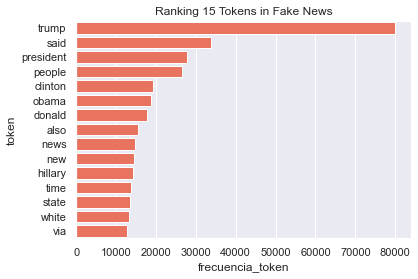
\includegraphics{output_63_0.png}
\caption{png}
\end{figure}

\begin{Shaded}
\begin{Highlighting}[]
\NormalTok{p2 }\OperatorTok{=}\NormalTok{ sns.barplot(data}\OperatorTok{=}\NormalTok{df\_no\_fake\_sort\_not\_StopWords.head(}\DecValTok{15}\NormalTok{), x}\OperatorTok{=}\StringTok{\textquotesingle{}frecuencia\_token\textquotesingle{}}\NormalTok{, y}\OperatorTok{=}\StringTok{\textquotesingle{}token\textquotesingle{}}\NormalTok{, color}\OperatorTok{=}\StringTok{\textquotesingle{}cyan\textquotesingle{}}\NormalTok{).}\BuiltInTok{set}\NormalTok{(title}\OperatorTok{=}\StringTok{\textquotesingle{}Ranking 15 Tokens in Not Fake News\textquotesingle{}}\NormalTok{) }
\end{Highlighting}
\end{Shaded}

\begin{figure}
\centering
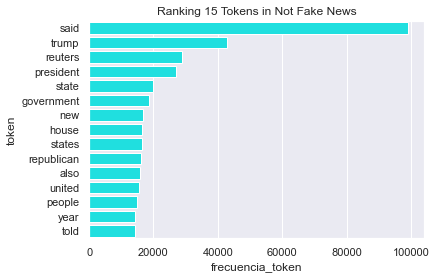
\includegraphics{output_64_0.png}
\caption{png}
\end{figure}

A continuación, se estudia qué palabras se utilizan de forma más
diferenciada en cada tipo de noticia (fake / no fake), es decir,
palabras que utiliza mucho en fake newa y que no se utilizan en las no
fakes, y viceversa.

Una forma de hacer este análisis es mediante el odds ratio de las
frecuencias.

\[\dfrac{ \frac{n_{k0} + 1}{N_0 + 1} }{  \frac{n_{k1} + 1}{N_1 +1}  }\]

Donde:

\(n_{k0}\) el número de veces que aparece el término (token) k en las
fake news

\(n_{k1}\) el numero de veces que aparece el termino (token) k en las no
fake news.

\(N_0\) es el número de terminos (tokens, contando repeticiones) que
aparecen en las fake news

\(N_1\) es el número de terminos (tokens, contando repeticiones) que
aparecen en las no fake news

\begin{Shaded}
\begin{Highlighting}[]
\KeywordTok{def}\NormalTok{ n\_k1(token) : }

\NormalTok{    n\_k1 }\OperatorTok{=}\NormalTok{ df\_fake\_sort\_not\_StopWords.loc[ df\_fake\_sort\_not\_StopWords[}\StringTok{\textquotesingle{}token\textquotesingle{}}\NormalTok{]}\OperatorTok{==}\NormalTok{token , }\StringTok{\textquotesingle{}frecuencia\_token\textquotesingle{}}\NormalTok{]}

    \ControlFlowTok{return}\NormalTok{(n\_k1)}
\end{Highlighting}
\end{Shaded}

\begin{Shaded}
\begin{Highlighting}[]
\KeywordTok{def}\NormalTok{ n\_k0(token) : }

\NormalTok{    n\_k0 }\OperatorTok{=}\NormalTok{ df\_no\_fake\_sort\_not\_StopWords.loc[ df\_no\_fake\_sort\_not\_StopWords[}\StringTok{\textquotesingle{}token\textquotesingle{}}\NormalTok{]}\OperatorTok{==}\NormalTok{token , }\StringTok{\textquotesingle{}frecuencia\_token\textquotesingle{}}\NormalTok{]}

    \ControlFlowTok{return}\NormalTok{(n\_k0)}
\end{Highlighting}
\end{Shaded}

\begin{Shaded}
\begin{Highlighting}[]
\NormalTok{n\_k0(}\StringTok{\textquotesingle{}trump\textquotesingle{}}\NormalTok{) }
\end{Highlighting}
\end{Shaded}

\begin{verbatim}
17    42755
Name: frecuencia_token, dtype: int64
\end{verbatim}

\begin{Shaded}
\begin{Highlighting}[]
\NormalTok{n\_k1(}\StringTok{\textquotesingle{}trump\textquotesingle{}}\NormalTok{) }
\end{Highlighting}
\end{Shaded}

\begin{verbatim}
10    79922
Name: frecuencia_token, dtype: int64
\end{verbatim}

N\_0 y N\_1 coinciden con el nº de tokens (contando repeticiones , y sin
stops words) que aparecen el las no fake y fake news, respectivamente:

\begin{Shaded}
\begin{Highlighting}[]
\NormalTok{Fake\_News\_Tokens\_not\_StopWords }\OperatorTok{=}\NormalTok{ Fake\_News\_Tokens[ }\OperatorTok{\textasciitilde{}}\NormalTok{ Fake\_News\_Tokens[}\StringTok{\textquotesingle{}token\textquotesingle{}}\NormalTok{].isin(stop\_words) ]}
\end{Highlighting}
\end{Shaded}

\begin{Shaded}
\begin{Highlighting}[]
\NormalTok{N0 }\OperatorTok{=}\NormalTok{ Fake\_News\_Tokens\_not\_StopWords.groupby(by}\OperatorTok{=}\StringTok{\textquotesingle{}Fake\textquotesingle{}}\NormalTok{)[}\StringTok{\textquotesingle{}token\textquotesingle{}}\NormalTok{].count()[}\DecValTok{0}\NormalTok{]}

\NormalTok{N1 }\OperatorTok{=}\NormalTok{ Fake\_News\_Tokens\_not\_StopWords.groupby(by}\OperatorTok{=}\StringTok{\textquotesingle{}Fake\textquotesingle{}}\NormalTok{)[}\StringTok{\textquotesingle{}token\textquotesingle{}}\NormalTok{].count()[}\DecValTok{1}\NormalTok{]}
\end{Highlighting}
\end{Shaded}

\begin{Shaded}
\begin{Highlighting}[]
\NormalTok{N0}
\end{Highlighting}
\end{Shaded}

\begin{verbatim}
4782198
\end{verbatim}

\begin{Shaded}
\begin{Highlighting}[]
\NormalTok{N1}
\end{Highlighting}
\end{Shaded}

\begin{verbatim}
5396339
\end{verbatim}

\begin{Shaded}
\begin{Highlighting}[]
\NormalTok{Fake\_News\_Tokens\_not\_StopWords.groupby(by}\OperatorTok{=}\StringTok{\textquotesingle{}Fake\textquotesingle{}}\NormalTok{)[}\StringTok{\textquotesingle{}token\textquotesingle{}}\NormalTok{].count()}
\end{Highlighting}
\end{Shaded}

\begin{verbatim}
Fake
0    4782198
1    5396339
Name: token, dtype: int64
\end{verbatim}

\begin{Shaded}
\begin{Highlighting}[]
\NormalTok{n\_k0(}\StringTok{\textquotesingle{}trump\textquotesingle{}}\NormalTok{) }\OperatorTok{/}\NormalTok{ N0 }
\end{Highlighting}
\end{Shaded}

\begin{verbatim}
17    0.00894
Name: frecuencia_token, dtype: float64
\end{verbatim}

\begin{Shaded}
\begin{Highlighting}[]
\NormalTok{n\_k1(}\StringTok{\textquotesingle{}trump\textquotesingle{}}\NormalTok{) }\OperatorTok{/}\NormalTok{ N1}
\end{Highlighting}
\end{Shaded}

\begin{verbatim}
10    0.01481
Name: frecuencia_token, dtype: float64
\end{verbatim}

\begin{Shaded}
\begin{Highlighting}[]
\BuiltInTok{float}\NormalTok{( n\_k0(}\StringTok{\textquotesingle{}trump\textquotesingle{}}\NormalTok{) }\OperatorTok{/}\NormalTok{ N0 ) }\OperatorTok{/} \BuiltInTok{float}\NormalTok{( n\_k1(}\StringTok{\textquotesingle{}trump\textquotesingle{}}\NormalTok{) }\OperatorTok{/}\NormalTok{ N1 )}
\end{Highlighting}
\end{Shaded}

\begin{verbatim}
0.6036597761892153
\end{verbatim}

\begin{Shaded}
\begin{Highlighting}[]
\NormalTok{df0 }\OperatorTok{=}\NormalTok{ df\_fake\_sort\_not\_StopWords.sort\_values(by}\OperatorTok{=}\NormalTok{[}\StringTok{"token"}\NormalTok{]).reset\_index(drop}\OperatorTok{=}\VariableTok{True}\NormalTok{)}
\NormalTok{df0}
\end{Highlighting}
\end{Shaded}

index

Fake

token

frecuencia\_token

0

125805

1

aa

24

1

125806

1

aaa

9

2

125807

1

aaaaaaaand

1

3

125808

1

aaaaackkk

1

4

125809

1

aaaaapkfhk

1

\ldots{}

\ldots{}

\ldots{}

\ldots{}

\ldots{}

125561

251605

1

''\,''it

0

125562

251606

1

''\,''when

0

125563

251607

1

•if

0

125564

251608

1

\(\surd\)

0

125565

251609

1

\(\Rightarrow\)

0

125566 rows × 4 columns

\begin{Shaded}
\begin{Highlighting}[]
\NormalTok{df1 }\OperatorTok{=}\NormalTok{ df\_no\_fake\_sort\_not\_StopWords.sort\_values(by}\OperatorTok{=}\NormalTok{[}\StringTok{"token"}\NormalTok{]).reset\_index(drop}\OperatorTok{=}\VariableTok{True}\NormalTok{)}
\NormalTok{df1}
\end{Highlighting}
\end{Shaded}

index

Fake

token

frecuencia\_token

0

0

0

aa

22

1

1

0

aaa

7

2

2

0

aaaaaaaand

0

3

3

0

aaaaackkk

0

4

4

0

aaaaapkfhk

0

\ldots{}

\ldots{}

\ldots{}

\ldots{}

\ldots{}

125561

125800

0

''\,''it

1

125562

125801

0

''\,''when

1

125563

125802

0

•if

3

125564

125803

0

\(\surd\)

3

125565

125804

0

\(\Rightarrow\)️

1

125566 rows × 4 columns

\begin{Shaded}
\begin{Highlighting}[]
\NormalTok{n\_k0\_vector }\OperatorTok{=}\NormalTok{ df0[}\StringTok{\textquotesingle{}frecuencia\_token\textquotesingle{}}\NormalTok{]}
\end{Highlighting}
\end{Shaded}

\begin{Shaded}
\begin{Highlighting}[]
\NormalTok{( n\_k0\_vector }\OperatorTok{+} \DecValTok{1}\NormalTok{ ) }\OperatorTok{/}\NormalTok{ ( N0 }\OperatorTok{+} \DecValTok{1}\NormalTok{)}
\end{Highlighting}
\end{Shaded}

\begin{verbatim}
0         5.227721e-06
1         2.091088e-06
2         4.182176e-07
3         4.182176e-07
4         4.182176e-07
              ...     
125561    2.091088e-07
125562    2.091088e-07
125563    2.091088e-07
125564    2.091088e-07
125565    2.091088e-07
Name: frecuencia_token, Length: 125566, dtype: float64
\end{verbatim}

\begin{Shaded}
\begin{Highlighting}[]
\NormalTok{n\_k1\_vector }\OperatorTok{=}\NormalTok{ df1[}\StringTok{\textquotesingle{}frecuencia\_token\textquotesingle{}}\NormalTok{]}
\end{Highlighting}
\end{Shaded}

\begin{Shaded}
\begin{Highlighting}[]
\NormalTok{( n\_k1\_vector }\OperatorTok{+} \DecValTok{1}\NormalTok{ ) }\OperatorTok{/}\NormalTok{ ( N1 }\OperatorTok{+} \DecValTok{1}\NormalTok{)}
\end{Highlighting}
\end{Shaded}

\begin{verbatim}
0         4.262148e-06
1         1.482486e-06
2         1.853108e-07
3         1.853108e-07
4         1.853108e-07
              ...     
125561    3.706216e-07
125562    3.706216e-07
125563    7.412431e-07
125564    7.412431e-07
125565    3.706216e-07
Name: frecuencia_token, Length: 125566, dtype: float64
\end{verbatim}

\begin{Shaded}
\begin{Highlighting}[]
\NormalTok{Odds\_ratio }\OperatorTok{=}\NormalTok{ ( ( n\_k0\_vector }\OperatorTok{+} \DecValTok{1}\NormalTok{ ) }\OperatorTok{/}\NormalTok{ ( N0 }\OperatorTok{+} \DecValTok{1}\NormalTok{) ) }\OperatorTok{/}\NormalTok{ ( ( n\_k1\_vector }\OperatorTok{+} \DecValTok{1}\NormalTok{ ) }\OperatorTok{/}\NormalTok{ ( N1 }\OperatorTok{+} \DecValTok{1}\NormalTok{) )}
\end{Highlighting}
\end{Shaded}

\begin{Shaded}
\begin{Highlighting}[]
\NormalTok{Odds\_ratio}
\end{Highlighting}
\end{Shaded}

\begin{verbatim}
0         1.226546
1         1.410528
2         2.256845
3         2.256845
4         2.256845
            ...   
125561    0.564211
125562    0.564211
125563    0.282106
125564    0.282106
125565    0.564211
Name: frecuencia_token, Length: 125566, dtype: float64
\end{verbatim}

\begin{Shaded}
\begin{Highlighting}[]
\NormalTok{df0[}\StringTok{\textquotesingle{}Odds\_ratio\_notFake\_Fake\textquotesingle{}}\NormalTok{] }\OperatorTok{=}\NormalTok{ Odds\_ratio  }
\NormalTok{df1[}\StringTok{\textquotesingle{}Odds\_ratio\_notFake\_Fake\textquotesingle{}}\NormalTok{] }\OperatorTok{=}\NormalTok{ Odds\_ratio  }
\end{Highlighting}
\end{Shaded}

\begin{Shaded}
\begin{Highlighting}[]
\NormalTok{df0}
\end{Highlighting}
\end{Shaded}

index

Fake

token

frecuencia\_token

Odds\_ratio\_notFake\_Fake

0

125805

1

aa

24

1.226546

1

125806

1

aaa

9

1.410528

2

125807

1

aaaaaaaand

1

2.256845

3

125808

1

aaaaackkk

1

2.256845

4

125809

1

aaaaapkfhk

1

2.256845

\ldots{}

\ldots{}

\ldots{}

\ldots{}

\ldots{}

\ldots{}

125561

251605

1

''\,''it

0

0.564211

125562

251606

1

''\,''when

0

0.564211

125563

251607

1

•if

0

0.282106

125564

251608

1

\(\surd\)

0

0.282106

125565

251609

1

\(\Rightarrrow\)/td\textgreater{}

0

\begin{verbatim}
  <td>0.564211</td>
</tr>
\end{verbatim}

125566 rows × 5 columns

\begin{Shaded}
\begin{Highlighting}[]
\NormalTok{df1}
\end{Highlighting}
\end{Shaded}

index

Fake

token

frecuencia\_token

Odds\_ratio\_notFake\_Fake

0

0

0

aa

22

1.226546

1

1

0

aaa

7

1.410528

2

2

0

aaaaaaaand

0

2.256845

3

3

0

aaaaackkk

0

2.256845

4

4

0

aaaaapkfhk

0

2.256845

\ldots{}

\ldots{}

\ldots{}

\ldots{}

\ldots{}

\ldots{}

125561

125800

0

''\,''it

1

0.564211

125562

125801

0

''\,''when

1

0.564211

125563

125802

0

•if

3

0.282106

125564

125803

0

\(\surd\)

3

0.282106

125565

125804

0

\(\Rightarrow\)

1

0.564211

125566 rows × 5 columns

\begin{Shaded}
\begin{Highlighting}[]
\NormalTok{df0 }\OperatorTok{=}\NormalTok{ df0.sort\_values(by}\OperatorTok{=}\NormalTok{[}\StringTok{"Odds\_ratio\_notFake\_Fake"}\NormalTok{], ascending}\OperatorTok{=}\VariableTok{False}\NormalTok{).reset\_index(drop}\OperatorTok{=}\VariableTok{True}\NormalTok{).head(}\DecValTok{15}\NormalTok{)}
\NormalTok{df0}
\end{Highlighting}
\end{Shaded}

index

Fake

token

frecuencia\_token

Odds\_ratio\_notFake\_Fake

0

161635

1

finicum

361

408.488873

1

240069

1

wikimedia

225

255.023440

2

234845

1

uninterruptible

213

241.482372

3

204177

1

philosophers

209

236.968683

4

186516

1

lovable

206

233.583416

5

193491

1

moralists

205

232.454994

6

223735

1

spore

205

232.454994

7

217054

1

savants

205

232.454994

8

210262

1

rascals

204

231.326572

9

189208

1

masochists

204

231.326572

10

158833

1

evangelists

204

231.326572

11

137313

1

boiler

778

219.760243

12

139559

1

bundy

770

217.503399

13

217966

1

screengrab

566

213.271815

14

239742

1

whined

187

212.143393

\begin{Shaded}
\begin{Highlighting}[]
\NormalTok{df1 }\OperatorTok{=}\NormalTok{ df1.sort\_values(by}\OperatorTok{=}\NormalTok{[}\StringTok{"Odds\_ratio\_notFake\_Fake"}\NormalTok{], ascending}\OperatorTok{=}\VariableTok{True}\NormalTok{).reset\_index(drop}\OperatorTok{=}\VariableTok{True}\NormalTok{).head(}\DecValTok{15}\NormalTok{)}
\NormalTok{df1[}\StringTok{\textquotesingle{}Odds\_ratio\_Fake\_notFake\textquotesingle{}}\NormalTok{] }\OperatorTok{=} \DecValTok{1} \OperatorTok{/}\NormalTok{ df1[}\StringTok{"Odds\_ratio\_notFake\_Fake"}\NormalTok{] }
\NormalTok{df1}
\end{Highlighting}
\end{Shaded}

index

Fake

token

frecuencia\_token

Odds\_ratio\_notFake\_Fake

Odds\_ratio\_Fake\_notFake

0

106864

0

trump's

11629

0.000097

10306.425164

1

72989

0

obama's

2132

0.000529

1890.249774

2

18791

0

clinton's

1604

0.000703

1422.339844

3

76630

0

party's

1101

0.001024

976.584740

4

98675

0

state's

1010

0.001116

895.941173

5

81106

0

president's

904

0.001247

802.004710

6

84132

0

rakhine

897

0.001257

795.801358

7

1245

0

administration's

765

0.001473

678.823876

8

88808

0

rohingya

2054

0.001647

607.042239

9

118151

0

zuma

682

0.001652

605.269853

10

82475

0

puigdemont

645

0.001747

572.480710

11

17557

0

china's

632

0.001783

560.960200

12

89850

0

russia's

615

0.001832

545.894918

13

21925

0

country's

574

0.001962

509.561003

14

69154

0

myanmar

2806

0.002010

497.508778

\begin{Shaded}
\begin{Highlighting}[]
\CommentTok{\#\#\# Alternativa computacionalmente mas costosa:}

\CommentTok{\# for token , i in zip( df\_fake\_sort\_sin\_StopWords[\textquotesingle{}token\textquotesingle{}] , range(0, len(df\_fake\_sort\_sin\_StopWords)) ):}

   \CommentTok{\# df\_fake\_sort\_sin\_StopWords[\textquotesingle{}Odds\_ratio\_notFake\_Fake\textquotesingle{}][i] = float( (n\_k0(token) + 1) / (N0 + 1) ) / float( (n\_k1(token) + 1) / (N1 + 1) )}

\CommentTok{\# for token , i in zip( df\_no\_fake\_sort\_sin\_StopWords[\textquotesingle{}token\textquotesingle{}] , range(0, len(df\_no\_fake\_sort\_sin\_StopWords)) ):}

   \CommentTok{\# df\_no\_fake\_sort\_sin\_StopWords[\textquotesingle{}Odds\_ratio\_notFake\_Fake\textquotesingle{}][i] = float( (n\_k0(token) + 1) / (N0 + 1) ) / float( (n\_k1(token) + 1) / (N1 + 1) )}
\end{Highlighting}
\end{Shaded}

\begin{Shaded}
\begin{Highlighting}[]
\NormalTok{p1 }\OperatorTok{=}\NormalTok{ sns.barplot(data}\OperatorTok{=}\NormalTok{df1.sort\_values(by}\OperatorTok{=}\NormalTok{[}\StringTok{"Odds\_ratio\_notFake\_Fake"}\NormalTok{], ascending}\OperatorTok{=}\VariableTok{True}\NormalTok{).reset\_index(drop}\OperatorTok{=}\VariableTok{True}\NormalTok{).head(}\DecValTok{15}\NormalTok{) ,}
\NormalTok{                 x}\OperatorTok{=}\StringTok{\textquotesingle{}Odds\_ratio\_Fake\_notFake\textquotesingle{}}\NormalTok{, y}\OperatorTok{=}\StringTok{\textquotesingle{}token\textquotesingle{}}\NormalTok{, color}\OperatorTok{=}\StringTok{\textquotesingle{}tomato\textquotesingle{}}\NormalTok{).}\BuiltInTok{set}\NormalTok{(title}\OperatorTok{=}\StringTok{\textquotesingle{}Ranking 15 most representative tokens in Fake News\textquotesingle{}}\NormalTok{) }
\end{Highlighting}
\end{Shaded}

\begin{figure}
\centering
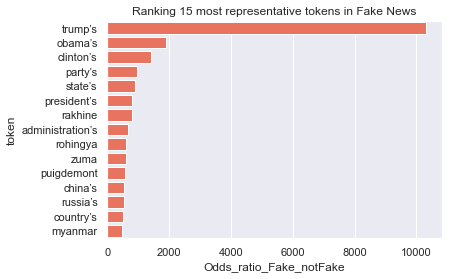
\includegraphics{output_95_0.png}
\caption{png}
\end{figure}

\begin{Shaded}
\begin{Highlighting}[]
\NormalTok{p2 }\OperatorTok{=}\NormalTok{ sns.barplot(data}\OperatorTok{=}\NormalTok{df0.sort\_values(by}\OperatorTok{=}\NormalTok{[}\StringTok{"Odds\_ratio\_notFake\_Fake"}\NormalTok{], ascending}\OperatorTok{=}\VariableTok{False}\NormalTok{).reset\_index(drop}\OperatorTok{=}\VariableTok{True}\NormalTok{).head(}\DecValTok{15}\NormalTok{) ,}
\NormalTok{                 x}\OperatorTok{=}\StringTok{\textquotesingle{}Odds\_ratio\_notFake\_Fake\textquotesingle{}}\NormalTok{, y}\OperatorTok{=}\StringTok{\textquotesingle{}token\textquotesingle{}}\NormalTok{, color}\OperatorTok{=}\StringTok{\textquotesingle{}cyan\textquotesingle{}}\NormalTok{).}\BuiltInTok{set}\NormalTok{(title}\OperatorTok{=}\StringTok{\textquotesingle{}Ranking 15 most representative tokens in Not Fake News\textquotesingle{}}\NormalTok{) }
\end{Highlighting}
\end{Shaded}

\begin{figure}
\centering
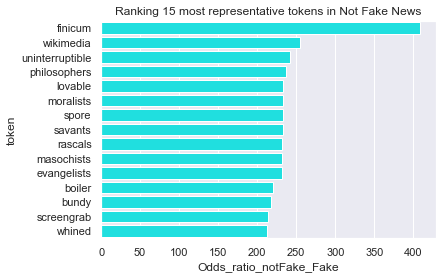
\includegraphics{output_96_0.png}
\caption{png}
\end{figure}

Uno de los principales intereses en text mining, natural language
processing e information retrieval es cuantificar la temática de un
texto, así como la importancia de cada término que lo forma. Una manera
sencilla de medir la importancia de un término dentro de un documento es
utilizando la frecuencia con la que aparece (tf, term-frequency). Esta
aproximación, aunque simple, tiene la limitación de atribuir mucha
importancia a aquellas palabras que aparecen muchas veces aunque no
aporten información selectiva. Por ejemplo, si la palabra matemáticas
aparece 5 veces en un documento y la palabra página aparece 50, la
segunda tendrá 10 veces más peso a pesar de que no aporte tanta
información sobre la temática del documento. Para solucionar este
problema se pueden ponderar los valores tf multiplicándolos por la
inversa de la frecuencia con la que el término en cuestión aparece en el
resto de documentos(idf). De esta forma, se consigue reducir el valor de
aquellos términos que aparecen en muchos documentos y que, por lo tanto,
no aportan información selectiva.

El estadístico tf-idf mide cómo de informativo es un término en un
documento teniendo en cuenta la frecuencia con la que ese término
aparece en otros documentos.

Term Frequency (tf)

\[tf (k, d)= \dfrac{n_k}{longitud( d)}\]

donde \(n_k\) es el número de veces que aparece el término \(k\) en el
documento \(d\) , y longitudd(d) es el nº de terminos del documento d

Inverse Document Frequency

\[idf (k)=log(\dfrac{n(d)}{n(d,k)})\]

donde \(n(d)\) es el número total de documentos y \(n(d,k)\) el número
de documentos que contienen el término \(k\) .

Estadístico tf-idf

\[tf\_idf(k, d)=tf (k, d)∗idf (k)\]

En la práctica, para evitar problemas con el logaritmo cuando aparecen
valores de 0, se emplea una versión corregida del idf (t) . Esta es la
versión implementada en Scikit Learn.

\[idf (k)=log(\dfrac{1+n(d)}{1+n(d,k)})+1\]

Calculo de tf

\begin{Shaded}
\begin{Highlighting}[]
\CommentTok{\# nº de veces que aparece cada termino (token) en cada noticia (n\_k)}

\NormalTok{df\_tf }\OperatorTok{=}\NormalTok{ pd.DataFrame( Fake\_News\_Tokens\_not\_StopWords.groupby([}\StringTok{\textquotesingle{}id\_text\textquotesingle{}}\NormalTok{,}\StringTok{\textquotesingle{}token\textquotesingle{}}\NormalTok{])[}\StringTok{\textquotesingle{}token\textquotesingle{}}\NormalTok{].count().reset\_index(name}\OperatorTok{=}\StringTok{\textquotesingle{}n\_k\textquotesingle{}}\NormalTok{) )}

\CommentTok{\# nº de terminos (tokens) en cada noticia (longitud(d))}

\NormalTok{df\_tf[}\StringTok{\textquotesingle{}longitud(d)\textquotesingle{}}\NormalTok{] }\OperatorTok{=}\NormalTok{ df\_tf.groupby(}\StringTok{\textquotesingle{}id\_text\textquotesingle{}}\NormalTok{)[}\StringTok{\textquotesingle{}n\_k\textquotesingle{}}\NormalTok{].transform(}\BuiltInTok{sum}\NormalTok{)}

\CommentTok{\# Calculo de term{-}frequency (tf)}

\NormalTok{df\_tf[}\StringTok{\textquotesingle{}tf\textquotesingle{}}\NormalTok{] }\OperatorTok{=}\NormalTok{ df\_tf[}\StringTok{\textquotesingle{}n\_k\textquotesingle{}}\NormalTok{] }\OperatorTok{/}\NormalTok{ df\_tf[}\StringTok{\textquotesingle{}longitud(d)\textquotesingle{}}\NormalTok{]}
\end{Highlighting}
\end{Shaded}

\begin{Shaded}
\begin{Highlighting}[]
\NormalTok{Fake\_News\_Tokens\_not\_StopWords.loc[Fake\_News\_Tokens\_not\_StopWords.token}\OperatorTok{==}\StringTok{\textquotesingle{}worth\textquotesingle{}}\NormalTok{]}
\end{Highlighting}
\end{Shaded}

id\_text

token

Fake

33

33

worth

1

36

36

worth

1

109

109

worth

1

147

147

worth

1

150

150

worth

1

\ldots{}

\ldots{}

\ldots{}

\ldots{}

44770

44770

worth

0

44849

44849

worth

0

44849

44849

worth

0

44897

44897

worth

0

44897

44897

worth

0

1687 rows × 3 columns

\begin{Shaded}
\begin{Highlighting}[]
\NormalTok{df\_tf}
\end{Highlighting}
\end{Shaded}

id\_text

token

n\_k

longitud(d)

tf

0

0

accept

1

251

0.003984

1

0

alan

1

251

0.003984

2

0

alansandoval

1

251

0.003984

3

0

allow

1

251

0.003984

4

0

also

1

251

0.003984

\ldots{}

\ldots{}

\ldots{}

\ldots{}

\ldots{}

\ldots{}

7155407

44897

union

1

132

0.007576

7155408

44897

volume

1

132

0.007576

7155409

44897

wants

1

132

0.007576

7155410

44897

worth

2

132

0.015152

7155411

44897

years

1

132

0.007576

7155412 rows × 5 columns

Calculo de Idf

\begin{Shaded}
\begin{Highlighting}[]
\CommentTok{\# Calculo del nº de documentos en los que aparece cada termino (token) (n(d,k))}

\NormalTok{df\_Idf }\OperatorTok{=}\NormalTok{ pd.DataFrame( Fake\_News\_Tokens\_not\_StopWords.groupby([}\StringTok{\textquotesingle{}token\textquotesingle{}}\NormalTok{])[}\StringTok{\textquotesingle{}id\_text\textquotesingle{}}\NormalTok{].nunique().reset\_index(name}\OperatorTok{=}\StringTok{\textquotesingle{}n\_d\_k\textquotesingle{}}\NormalTok{) )}

\CommentTok{\# Ojo, si se usa count en lugar de nunique no se estaria contando el nº de documentos}
\CommentTok{\# en los que aparece cada termino, si no el nº de veces en total (contando repeticiones) que}
\CommentTok{\# aparece un termino en el conjunto de documentos. Por ejemplo, dado un termino k que aparece}
\CommentTok{\# 10 veces en el documento d1 y 3 veces en el d4 , usando count() la cuenta sale 13 , que es el }
\CommentTok{\# nº de veces que aparece k en el conjunto de los documentos, en cambio usando nunique()}
\CommentTok{\#  la cuenta sale 2 que es el nº de documentos en los que aparece el termino k, que es lo que buscamos}

\CommentTok{\# Calculo del nº total de documentos (n\_d)}

\NormalTok{df\_Idf[}\StringTok{\textquotesingle{}n\_d\textquotesingle{}}\NormalTok{] }\OperatorTok{=} \BuiltInTok{len}\NormalTok{(Fake\_News\_Data)}

\CommentTok{\# Calculo de Idf}

\NormalTok{df\_Idf[}\StringTok{\textquotesingle{}Idf\textquotesingle{}}\NormalTok{] }\OperatorTok{=}\NormalTok{ np.log( (df\_Idf[}\StringTok{\textquotesingle{}n\_d\textquotesingle{}}\NormalTok{] ) }\OperatorTok{/}\NormalTok{ (df\_Idf[}\StringTok{\textquotesingle{}n\_d\_k\textquotesingle{}}\NormalTok{]) ) }\OperatorTok{+} \DecValTok{1} 
\end{Highlighting}
\end{Shaded}

\begin{Shaded}
\begin{Highlighting}[]
\NormalTok{df\_Idf}
\end{Highlighting}
\end{Shaded}

token

n\_d\_k

n\_d

Idf

0

aa

28

44898

8.379944

1

aaa

11

44898

9.314253

2

aaaaaaaand

1

44898

11.712149

3

aaaaackkk

1

44898

11.712149

4

aaaaapkfhk

1

44898

11.712149

\ldots{}

\ldots{}

\ldots{}

\ldots{}

\ldots{}

125561

''\,''it

1

44898

11.712149

125562

''\,''when

1

44898

11.712149

125563

•if

1

44898

11.712149

125564

☑️

1

44898

11.712149

125565

\(\Rightarrow\)

1

44898

11.712149

125566 rows × 4 columns

Calculo de tf-Idf

\begin{Shaded}
\begin{Highlighting}[]
\NormalTok{df\_tf\_Idf }\OperatorTok{=}\NormalTok{ pd.merge(df\_tf, df\_Idf, on}\OperatorTok{=}\StringTok{\textquotesingle{}token\textquotesingle{}}\NormalTok{)}

\NormalTok{df\_tf\_Idf[}\StringTok{\textquotesingle{}tf\_Idf\textquotesingle{}}\NormalTok{] }\OperatorTok{=}\NormalTok{ df\_tf\_Idf[}\StringTok{\textquotesingle{}tf\textquotesingle{}}\NormalTok{] }\OperatorTok{*}\NormalTok{ df\_tf\_Idf[}\StringTok{\textquotesingle{}Idf\textquotesingle{}}\NormalTok{] }

\NormalTok{df\_tf\_Idf }\OperatorTok{=}\NormalTok{ df\_tf\_Idf.sort\_values(by}\OperatorTok{=}\StringTok{"id\_text"}\NormalTok{)}
\end{Highlighting}
\end{Shaded}

\begin{Shaded}
\begin{Highlighting}[]
\NormalTok{df\_tf\_Idf}
\end{Highlighting}
\end{Shaded}

id\_text

token

n\_k

longitud(d)

tf

n\_d\_k

n\_d

Idf

tf\_Idf

0

0

accept

1

251

0.003984

1395

44898

4.471499

0.017815

304262

0

pollitt

1

251

0.003984

1

44898

11.712149

0.046662

304263

0

power

1

251

0.003984

5057

44898

3.183620

0.012684

309320

0

president

3

251

0.011952

23571

44898

1.644376

0.019654

332891

0

presidential

1

251

0.003984

8823

44898

2.627031

0.010466

\ldots{}

\ldots{}

\ldots{}

\ldots{}

\ldots{}

\ldots{}

\ldots{}

\ldots{}

\ldots{}

\ldots{}

5516302

44897

amid

1

132

0.007576

1316

44898

4.529796

0.034317

5350014

44897

string

1

132

0.007576

404

44898

5.710734

0.043263

2043348

44897

state

2

132

0.015152

14226

44898

2.149322

0.032565

1423490

44897

delivered

1

132

0.007576

882

44898

4.929956

0.037348

7155411

44897

suhkoi

1

132

0.007576

1

44898

11.712149

0.088728

7155412 rows × 9 columns

Puede observarse que para la primera noticia (id\_text = 0), todos los
términos que aparecen una vez, tienen el mismo valor de tf, sin embargo,
dado que no todos los términos aparecen con la misma frecuencia en el
conjunto de todas las noticias, la corrección de idf es distinta para
cada uno.

\begin{Shaded}
\begin{Highlighting}[]
\NormalTok{df\_tf\_Idf.loc[df\_tf\_Idf.id\_text }\OperatorTok{==} \DecValTok{0}\NormalTok{ , ].sort\_values([}\StringTok{\textquotesingle{}tf\_Idf\textquotesingle{}}\NormalTok{], ascending}\OperatorTok{=}\VariableTok{False}\NormalTok{).head(}\DecValTok{10}\NormalTok{)}
\end{Highlighting}
\end{Shaded}

id\_text

token

n\_k

longitud(d)

tf

n\_d\_k

n\_d

Idf

tf\_Idf

90877

0

december

13

251

0.051793

2124

44898

4.051092

0.209818

152076

0

haters

6

251

0.023904

117

44898

6.949975

0.166135

439903

0

year

15

251

0.059761

13949

44898

2.168985

0.129621

148808

0

happy

6

251

0.023904

1151

44898

4.663762

0.111484

113622

0

enemies

5

251

0.019920

502

44898

5.493548

0.109433

427231

0

wish

5

251

0.019920

781

44898

5.051573

0.100629

245784

0

new

11

251

0.043825

15771

44898

2.046220

0.089675

233923

0

marlene

2

251

0.007968

9

44898

9.514924

0.075816

94857

0

dishonest

3

251

0.011952

269

44898

6.117437

0.073117

378476

0

trump

9

251

0.035857

21690

44898

1.727542

0.061944

\begin{Shaded}
\begin{Highlighting}[]
\NormalTok{df\_tf\_Idf.loc[df\_tf\_Idf.id\_text }\OperatorTok{==} \DecValTok{0}\NormalTok{ , ].sort\_values([}\StringTok{\textquotesingle{}tf\_Idf\textquotesingle{}}\NormalTok{], ascending}\OperatorTok{=}\VariableTok{True}\NormalTok{).head(}\DecValTok{10}\NormalTok{)}
\end{Highlighting}
\end{Shaded}

id\_text

token

n\_k

longitud(d)

tf

n\_d\_k

n\_d

Idf

tf\_Idf

4642

0

also

1

251

0.003984

18673

44898

1.877315

0.007479

193583

0

last

1

251

0.003984

14292

44898

2.144693

0.008545

347328

0

say

1

251

0.003984

10630

44898

2.440713

0.009724

223346

0

make

1

251

0.003984

10577

44898

2.445711

0.009744

121755

0

former

1

251

0.003984

10469

44898

2.455975

0.009785

162356

0

including

1

251

0.003984

9455

44898

2.557850

0.010191

33580

0

american

1

251

0.003984

9421

44898

2.561452

0.010205

332891

0

presidential

1

251

0.003984

8823

44898

2.627031

0.010466

181991

0

know

1

251

0.003984

8321

44898

2.685611

0.010700

404999

0

twitter

1

251

0.003984

7217

44898

2.827954

0.011267

\begin{Shaded}
\begin{Highlighting}[]
\NormalTok{df\_tf\_Idf.loc[df\_tf\_Idf.id\_text }\OperatorTok{==} \DecValTok{100}\NormalTok{ , ].sort\_values([}\StringTok{\textquotesingle{}tf\_Idf\textquotesingle{}}\NormalTok{], ascending}\OperatorTok{=}\VariableTok{False}\NormalTok{).head(}\DecValTok{10}\NormalTok{)}
\end{Highlighting}
\end{Shaded}

id\_text

token

n\_k

longitud(d)

tf

n\_d\_k

n\_d

Idf

tf\_Idf

5020628

100

biden

11

183

0.060109

371

44898

5.795946

0.348390

1574616

100

well

10

183

0.054645

9174

44898

2.588020

0.141422

378563

100

trump

13

183

0.071038

21690

44898

1.727542

0.122722

5021820

100

maples

2

183

0.010929

18

44898

8.821777

0.096413

3594634

100

married

3

183

0.016393

559

44898

5.385999

0.088295

5021747

100

lauer

2

183

0.010929

73

44898

7.421689

0.081111

4418334

100

marry

2

183

0.010929

114

44898

6.975950

0.076240

1087111

100

think

5

183

0.027322

8239

44898

2.695514

0.073648

1722158

100

something

4

183

0.021858

5041

44898

3.186789

0.069657

4551752

100

grow

2

183

0.010929

589

44898

5.333722

0.058292

\begin{Shaded}
\begin{Highlighting}[]
\NormalTok{df\_tf\_Idf.loc[df\_tf\_Idf.id\_text }\OperatorTok{==} \DecValTok{100}\NormalTok{ , ].sort\_values([}\StringTok{\textquotesingle{}tf\_Idf\textquotesingle{}}\NormalTok{], ascending}\OperatorTok{=}\VariableTok{True}\NormalTok{).head(}\DecValTok{10}\NormalTok{)}
\end{Highlighting}
\end{Shaded}

id\_text

token

n\_k

longitud(d)

tf

n\_d\_k

n\_d

Idf

tf\_Idf

1103859

100

time

1

183

0.005464

13972

44898

2.167338

0.011843

439938

100

year

1

183

0.005464

13949

44898

2.168985

0.011852

1202811

100

first

1

183

0.005464

12458

44898

2.282030

0.012470

261592

100

news

1

183

0.005464

11498

44898

2.362220

0.012908

1275844

100

obama

1

183

0.005464

9438

44898

2.559649

0.013987

1021277

100

right

1

183

0.005464

9400

44898

2.563684

0.014009

2267723

100

take

1

183

0.005464

9223

44898

2.582693

0.014113

1850090

100

office

1

183

0.005464

8155

44898

2.705762

0.014786

405046

100

twitter

1

183

0.005464

7217

44898

2.827954

0.015453

2949266

100

asked

1

183

0.005464

7116

44898

2.842047

0.015530

Clasificacion de texto:

Para poder aplicar algoritmos de clasificación a un texto, es necesario
crear una representación numérica del mismo. Una de las formas más
utilizadas se conoce como Bag of Words. Este método consiste en
identificar el set formado por todas las palabras (tokens) que aparecen
en el corpus, en este caso el conjunto de todos los tweets recuperados.
Con este set se crea un espacio n-dimensional en el que cada dimensión
(columna) es una palabra. Por último, se proyecta cada texto en ese
espacio, asignando un valor para cada dimensión. En la mayoría de casos,
el valor utilizado es el tf-idf.

Para facilitar la obtención de la matriz TF-IDF se recurre a la clase
TfidVectorized también de Scikit-Learn pero, en lugar de utilizar el
tokenizador por defecto, se emplea el mismo definido en los apartados
anteriores.

\begin{Shaded}
\begin{Highlighting}[]
\NormalTok{Fake\_News\_Tokens\_not\_StopWords[}\StringTok{\textquotesingle{}token\textquotesingle{}}\NormalTok{].nunique()}
\end{Highlighting}
\end{Shaded}

\begin{verbatim}
125566
\end{verbatim}

tokens = pd.DataFrame(
Fake\_News\_Tokens\_not\_StopWords{[}`token'{]}.unique()
).sort\_values({[}0{]}){[}0{]}

TF\_IDF\_Matrix = pd.DataFrame( 0 , index=range(0,
len(Fake\_News\_Data)) , columns=tokens )

i = 0

for k in range(0, len(df.loc{[} (df{[}`id\_text'{]}==i) , : {]})):

\begin{verbatim}
token = df.loc[ (df['id_text']==i) , 'token' ][k]

for j in range(0, TF_IDF_Matrix.shape[1]):

    if TF_IDF_Matrix.columns[j] == token :

        TF_IDF_Matrix.iloc[i , j] = df.loc[ (df['id_text']==i) & (df['token']== token ), 'tf_Idf' ]
\end{verbatim}

\begin{Shaded}
\begin{Highlighting}[]
\NormalTok{df }\OperatorTok{=}\NormalTok{ df\_tf\_Idf.loc[: , [}\StringTok{\textquotesingle{}id\_text\textquotesingle{}}\NormalTok{, }\StringTok{\textquotesingle{}token\textquotesingle{}}\NormalTok{, }\StringTok{\textquotesingle{}tf\_Idf\textquotesingle{}}\NormalTok{]]}

\NormalTok{df}
\end{Highlighting}
\end{Shaded}

id\_text

token

tf\_Idf

0

0

accept

0.017815

304262

0

pollitt

0.046662

304263

0

power

0.012684

309320

0

president

0.019654

332891

0

presidential

0.010466

\ldots{}

\ldots{}

\ldots{}

\ldots{}

5516302

44897

amid

0.034317

5350014

44897

string

0.043263

2043348

44897

state

0.032565

1423490

44897

delivered

0.037348

7155411

44897

suhkoi

0.088728

7155412 rows × 3 columns

TF\_IDF Matrix con sklearn

\begin{Shaded}
\begin{Highlighting}[]
\NormalTok{X\_data }\OperatorTok{=}\NormalTok{ Fake\_News\_Data.loc[ : , }\StringTok{\textquotesingle{}text\textquotesingle{}}\NormalTok{]}
\NormalTok{X\_data}
\end{Highlighting}
\end{Shaded}

\begin{verbatim}
0        Donald Trump just couldn t wish all Americans ...
1        House Intelligence Committee Chairman Devin Nu...
2        On Friday, it was revealed that former Milwauk...
3        On Christmas day, Donald Trump announced that ...
4        Pope Francis used his annual Christmas Day mes...
                               ...                        
44893    BRUSSELS (Reuters) - NATO allies on Tuesday we...
44894    LONDON (Reuters) - LexisNexis, a provider of l...
44895    MINSK (Reuters) - In the shadow of disused Sov...
44896    MOSCOW (Reuters) - Vatican Secretary of State ...
44897    JAKARTA (Reuters) - Indonesia will buy 11 Sukh...
Name: text, Length: 44898, dtype: object
\end{verbatim}

\begin{Shaded}
\begin{Highlighting}[]
\NormalTok{Y\_data }\OperatorTok{=}\NormalTok{ Fake\_News\_Data.loc[ : , }\StringTok{\textquotesingle{}Fake\textquotesingle{}}\NormalTok{]}
\NormalTok{Y\_data}
\end{Highlighting}
\end{Shaded}

\begin{verbatim}
0        1
1        1
2        1
3        1
4        1
        ..
44893    0
44894    0
44895    0
44896    0
44897    0
Name: Fake, Length: 44898, dtype: object
\end{verbatim}

\begin{Shaded}
\begin{Highlighting}[]
\ImportTok{from}\NormalTok{ sklearn.feature\_extraction.text }\ImportTok{import}\NormalTok{ TfidfVectorizer}
\end{Highlighting}
\end{Shaded}

\begin{Shaded}
\begin{Highlighting}[]
\NormalTok{tfidf\_vectorizador }\OperatorTok{=}\NormalTok{ TfidfVectorizer(tokenizer  }\OperatorTok{=}\NormalTok{ limpiar\_tokenizar, min\_df }\OperatorTok{=} \DecValTok{0}\NormalTok{, stop\_words }\OperatorTok{=}\NormalTok{ stop\_words, smooth\_idf}\OperatorTok{=}\VariableTok{False}\NormalTok{)}
\end{Highlighting}
\end{Shaded}

\begin{Shaded}
\begin{Highlighting}[]
\NormalTok{tfidf\_vectorizador.fit(X\_data)}
\end{Highlighting}
\end{Shaded}

\begin{verbatim}
c:\Users\Usuario\AppData\Local\Programs\Python\Python310\lib\site-packages\sklearn\feature_extraction\text.py:516: UserWarning: The parameter 'token_pattern' will not be used since 'tokenizer' is not None'
  warnings.warn(





TfidfVectorizer(min_df=0, smooth_idf=False,
                stop_words=['i', 'me', 'my', 'myself', 'we', 'our', 'ours',
                            'ourselves', 'you', "you're", "you've", "you'll",
                            "you'd", 'your', 'yours', 'yourself', 'yourselves',
                            'he', 'him', 'his', 'himself', 'she', "she's",
                            'her', 'hers', 'herself', 'it', "it's", 'its',
                            'itself', ...],
                tokenizer=<function limpiar_tokenizar at 0x00000245F12E6290>)
\end{verbatim}

\begin{Shaded}
\begin{Highlighting}[]
\NormalTok{tfidf\_matrix }\OperatorTok{=}\NormalTok{ tfidf\_vectorizador.transform(X\_data)}
\end{Highlighting}
\end{Shaded}

\begin{Shaded}
\begin{Highlighting}[]
\NormalTok{tfidf\_matrix.shape}
\end{Highlighting}
\end{Shaded}

\begin{verbatim}
(44898, 125566)
\end{verbatim}

\begin{Shaded}
\begin{Highlighting}[]
\BuiltInTok{print}\NormalTok{(tfidf\_vectorizador.get\_feature\_names\_out()[}\DecValTok{0}\NormalTok{:}\DecValTok{50}\NormalTok{])}
\end{Highlighting}
\end{Shaded}

\begin{verbatim}
['aa' 'aaa' 'aaaaaaaand' 'aaaaackkk' 'aaaaapkfhk' 'aaaahhhh' 'aaaand'
 'aaaarrgh' 'aaab' 'aaarf' 'aab' 'aaba' 'aabfsv' 'aabge' 'aabo'
 'aaccording' 'aachen' 'aacnr' 'aadhaar' 'aadhar' 'aadl' 'aaf' 'aafn'
 'aag' 'aahd' 'aahwuhvvnh' 'aai' 'aaj' 'aaja' 'aal' 'aalberg' 'aalberts'
 'aaldef' 'aaliyah' 'aamer' 'aamin' 'aammir' 'aamom' 'aamrrd' 'aan'
 'aaofj' 'aapa' 'aapi' 'aapl' 'aapxim' 'aar' 'aardal' 'aardvark'
 'aardvarks' 'aargh']
\end{verbatim}

\begin{Shaded}
\begin{Highlighting}[]
\NormalTok{tfidf\_vectorizador.get\_feature\_names\_out()[}\DecValTok{10}\NormalTok{]}
\end{Highlighting}
\end{Shaded}

\begin{verbatim}
'aab'
\end{verbatim}

\begin{Shaded}
\begin{Highlighting}[]
\NormalTok{df\_index\_token }\OperatorTok{=}\NormalTok{ pd.DataFrame( \{}\StringTok{\textquotesingle{}index\textquotesingle{}}\NormalTok{ : }\BuiltInTok{range}\NormalTok{(}\DecValTok{0}\NormalTok{, }\BuiltInTok{len}\NormalTok{(tfidf\_vectorizador.get\_feature\_names\_out())) , }\StringTok{\textquotesingle{}token\textquotesingle{}}\NormalTok{ : tfidf\_vectorizador.get\_feature\_names\_out() \})}
\end{Highlighting}
\end{Shaded}

\begin{Shaded}
\begin{Highlighting}[]
\NormalTok{df\_index\_token}
\end{Highlighting}
\end{Shaded}

index

token

0

0

aa

1

1

aaa

2

2

aaaaaaaand

3

3

aaaaackkk

4

4

aaaaapkfhk

\ldots{}

\ldots{}

\ldots{}

125561

125561

''\,''it

125562

125562

''\,''when

125563

125563

•if

125564

125564

☑️

125565

125565

\(\Rightarrow\)

125566 rows × 2 columns

\begin{Shaded}
\begin{Highlighting}[]
\NormalTok{df\_index\_token.loc[df\_index\_token.token }\OperatorTok{==} \StringTok{\textquotesingle{}accept\textquotesingle{}}\NormalTok{, ]}
\end{Highlighting}
\end{Shaded}

index

token

645

645

accept

\begin{Shaded}
\begin{Highlighting}[]
\NormalTok{df\_index\_token.loc[df\_index\_token.token }\OperatorTok{==} \StringTok{\textquotesingle{}pollitt\textquotesingle{}}\NormalTok{, ]}
\end{Highlighting}
\end{Shaded}

index

token

79741

79741

pollitt

\begin{Shaded}
\begin{Highlighting}[]
\NormalTok{df\_index\_token.loc[df\_index\_token.token }\OperatorTok{==} \StringTok{\textquotesingle{}pollitt\textquotesingle{}}\NormalTok{, ]}
\end{Highlighting}
\end{Shaded}

index

token

79741

79741

pollitt

\begin{Shaded}
\begin{Highlighting}[]
\NormalTok{tfidf\_matrix[}\DecValTok{0}\NormalTok{, }\DecValTok{645}\NormalTok{]}
\end{Highlighting}
\end{Shaded}

\begin{verbatim}
0.034889784479772486
\end{verbatim}

\begin{Shaded}
\begin{Highlighting}[]
\FloatTok{0.034889784479772486}\OperatorTok{/}\FloatTok{0.017815}
\end{Highlighting}
\end{Shaded}

\begin{verbatim}
1.958449872566516
\end{verbatim}

\begin{Shaded}
\begin{Highlighting}[]
\NormalTok{tfidf\_matrix[}\DecValTok{0}\NormalTok{, }\DecValTok{79741}\NormalTok{]}
\end{Highlighting}
\end{Shaded}

\begin{verbatim}
0.09138643507615184
\end{verbatim}

\begin{Shaded}
\begin{Highlighting}[]
\FloatTok{0.09138643507615184}\OperatorTok{/}\FloatTok{0.046662}
\end{Highlighting}
\end{Shaded}

\begin{verbatim}
1.958476599291754
\end{verbatim}

\begin{Shaded}
\begin{Highlighting}[]
\NormalTok{df\_index\_token.loc[df\_index\_token.token }\OperatorTok{==} \StringTok{\textquotesingle{}string\textquotesingle{}}\NormalTok{, ]}
\end{Highlighting}
\end{Shaded}

index

token

99546

99546

string

\begin{Shaded}
\begin{Highlighting}[]
\NormalTok{tfidf\_matrix[}\DecValTok{44897}\NormalTok{, }\DecValTok{99546}\NormalTok{]}
\end{Highlighting}
\end{Shaded}

\begin{verbatim}
0.07393279140214064
\end{verbatim}

\begin{Shaded}
\begin{Highlighting}[]
\FloatTok{0.07393279140214064} \OperatorTok{/} \FloatTok{0.043263}
\end{Highlighting}
\end{Shaded}

\begin{verbatim}
1.708915040615321
\end{verbatim}

\begin{Shaded}
\begin{Highlighting}[]
\NormalTok{df\_index\_token.loc[df\_index\_token.token }\OperatorTok{==} \StringTok{\textquotesingle{}suhkoi\textquotesingle{}}\NormalTok{, ]}
\end{Highlighting}
\end{Shaded}

index

token

100181

100181

suhkoi

\begin{Shaded}
\begin{Highlighting}[]
\NormalTok{tfidf\_matrix[}\DecValTok{44897}\NormalTok{, }\DecValTok{100181}\NormalTok{]}
\end{Highlighting}
\end{Shaded}

\begin{verbatim}
0.15162882511320822
\end{verbatim}

\begin{Shaded}
\begin{Highlighting}[]
\FloatTok{0.15162882511320822} \OperatorTok{/} \FloatTok{0.088728}
\end{Highlighting}
\end{Shaded}

\begin{verbatim}
1.7089174230593298
\end{verbatim}

\begin{Shaded}
\begin{Highlighting}[]
\NormalTok{df\_index\_token.loc[df\_index\_token.token }\OperatorTok{==} \StringTok{\textquotesingle{}black\textquotesingle{}}\NormalTok{, ]}
\end{Highlighting}
\end{Shaded}

index

token

10627

10627

black

\begin{Shaded}
\begin{Highlighting}[]
\NormalTok{tfidf\_matrix[}\DecValTok{2}\NormalTok{, }\DecValTok{10627}\NormalTok{]}
\end{Highlighting}
\end{Shaded}

\begin{verbatim}
0.06661863120241834
\end{verbatim}

\begin{Shaded}
\begin{Highlighting}[]
\FloatTok{0.06661863120241834} \OperatorTok{/} \FloatTok{0.032256}
\end{Highlighting}
\end{Shaded}

\begin{verbatim}
2.065309747098783
\end{verbatim}

\begin{Shaded}
\begin{Highlighting}[]
\NormalTok{df\_index\_token.loc[df\_index\_token.token }\OperatorTok{==} \StringTok{\textquotesingle{}never\textquotesingle{}}\NormalTok{, ]}
\end{Highlighting}
\end{Shaded}

index

token

70560

70560

never

\begin{Shaded}
\begin{Highlighting}[]
\NormalTok{tfidf\_matrix[}\DecValTok{3}\NormalTok{, }\DecValTok{70560}\NormalTok{]}
\end{Highlighting}
\end{Shaded}

\begin{verbatim}
0.022176846230040667
\end{verbatim}

\begin{Shaded}
\begin{Highlighting}[]
\FloatTok{0.022176846230040674} \OperatorTok{/} \FloatTok{0.012048}
\end{Highlighting}
\end{Shaded}

\begin{verbatim}
1.8407076884163907
\end{verbatim}

\begin{Shaded}
\begin{Highlighting}[]
\NormalTok{tfidf\_matrix[}\DecValTok{55}\NormalTok{, }\DecValTok{38169}\NormalTok{]}
\end{Highlighting}
\end{Shaded}

\begin{verbatim}
0.03875545076716381
\end{verbatim}

\begin{Shaded}
\begin{Highlighting}[]
\FloatTok{0.038755450767163815} \OperatorTok{/} \FloatTok{0.018234}
\end{Highlighting}
\end{Shaded}

\begin{verbatim}
2.12544975140747
\end{verbatim}

\begin{Shaded}
\begin{Highlighting}[]
\NormalTok{df\_index\_token.loc[df\_index\_token.token }\OperatorTok{==} \StringTok{\textquotesingle{}dinner\textquotesingle{}}\NormalTok{, ]}
\end{Highlighting}
\end{Shaded}

index

token

26892

26892

dinner

\begin{Shaded}
\begin{Highlighting}[]
\NormalTok{tfidf\_matrix[}\DecValTok{240}\NormalTok{, }\DecValTok{26892}\NormalTok{]}
\end{Highlighting}
\end{Shaded}

\begin{verbatim}
0.1321697134106531
\end{verbatim}

\begin{Shaded}
\begin{Highlighting}[]
\FloatTok{0.1321697134106531} \OperatorTok{/} \FloatTok{0.064895}
\end{Highlighting}
\end{Shaded}

\begin{verbatim}
2.0366702120448896
\end{verbatim}

\begin{Shaded}
\begin{Highlighting}[]
\NormalTok{df\_index\_token.loc[df\_index\_token.token }\OperatorTok{==} \StringTok{\textquotesingle{}investigation\textquotesingle{}}\NormalTok{, ]}
\end{Highlighting}
\end{Shaded}

index

token

50314

50314

investigation

\begin{Shaded}
\begin{Highlighting}[]
\NormalTok{tfidf\_matrix[}\DecValTok{1522}\NormalTok{, }\DecValTok{50314}\NormalTok{]}
\end{Highlighting}
\end{Shaded}

\begin{verbatim}
0.2598673157066844
\end{verbatim}

\begin{Shaded}
\begin{Highlighting}[]
\FloatTok{0.25986731570668453} \OperatorTok{/} \FloatTok{0.116061}
\end{Highlighting}
\end{Shaded}

\begin{verbatim}
2.2390580445342065
\end{verbatim}

\begin{Shaded}
\begin{Highlighting}[]
\NormalTok{df\_tf\_Idf.loc[df\_tf\_Idf.id\_text}\OperatorTok{==}\DecValTok{1522}\NormalTok{, :]}
\end{Highlighting}
\end{Shaded}

id\_text

token

n\_k

longitud(d)

tf

n\_d\_k

n\_d

Idf

tf\_Idf

5491898

1522

worried

1

210

0.004762

1035

44898

4.769992

0.022714

3581331

1522

animal

1

210

0.004762

168

44898

6.588185

0.031372

4277714

1522

filing

1

210

0.004762

472

44898

5.555170

0.026453

6495797

1522

assurance

1

210

0.004762

67

44898

7.507456

0.035750

4015679

1522

investigating

1

210

0.004762

1233

44898

4.594943

0.021881

\ldots{}

\ldots{}

\ldots{}

\ldots{}

\ldots{}

\ldots{}

\ldots{}

\ldots{}

\ldots{}

\ldots{}

2646944

1522

increasingly

1

210

0.004762

1045

44898

4.760376

0.022668

635701

1522

investigation

7

210

0.033333

3753

44898

3.481838

0.116061

2960920

1522

claiming

1

210

0.004762

1198

44898

4.623740

0.022018

1872097

1522

probe

2

210

0.009524

1064

44898

4.742358

0.045165

3005817

1522

requested

1

210

0.004762

730

44898

5.119104

0.024377

151 rows × 9 columns

Como vemos, la metrica calculada por sklearn pese a que ne teoria es el
tf\_idf calculado con las formulas antes descritas, parece ser el doble
de nuestra metrica calculada (aunque esta cantidad varia en funcion del
documento considerado, pero esta entre 1.7 y 2.3 segun nuestras
pruebas). En cualquier caso lo importante es que tanto si sklearn
calcula correctamente el tf\_idf y nosotros nos hemos equivocado (que es
lo mas porbable), como si nosotros lo hemos calculado bien y sklearn ha
usado realmente otra version de la formula, en cualquier caso, nuestra
metriaca seria proporcional al verrdadero tf\_idf (si nosotros estamos
``errando'') o la de sklearn lo seria (si ellos ``erran'')

Asi que la matriz que devuelve sklearn nos es util pese a las
discrepacias de valores, porque es en cualquier caso proporcional.

\begin{Shaded}
\begin{Highlighting}[]
\NormalTok{tfidf\_matrix }\OperatorTok{=}\NormalTok{ tfidf\_vectorizador.fit\_transform(X\_data.iloc[}\DecValTok{0}\NormalTok{:}\DecValTok{2000}\NormalTok{,])}
\end{Highlighting}
\end{Shaded}

\begin{Shaded}
\begin{Highlighting}[]
\NormalTok{tfidf\_df}\OperatorTok{=}\NormalTok{ pd.DataFrame(tfidf\_matrix.todense())  }
\NormalTok{tfidf\_df.columns }\OperatorTok{=}\NormalTok{ tfidf\_vectorizador.get\_feature\_names()}
\end{Highlighting}
\end{Shaded}

\begin{verbatim}
c:\Users\Usuario\AppData\Local\Programs\Python\Python310\lib\site-packages\sklearn\utils\deprecation.py:87: FutureWarning: Function get_feature_names is deprecated; get_feature_names is deprecated in 1.0 and will be removed in 1.2. Please use get_feature_names_out instead.
  warnings.warn(msg, category=FutureWarning)
\end{verbatim}

\begin{Shaded}
\begin{Highlighting}[]
\NormalTok{tfidf\_df}
\end{Highlighting}
\end{Shaded}

aa

aaaand

aacnr

aaj

aaliyah

aaofj

aargh

aaron

aaroncovfefe

aaronshhh

\ldots{}

zxf

zy

zyf

zyklon

zz

zzlo

zzomtmd

zztaine

zzzzaaaacccchhh

zzzzzzzzzzzzz

0

0.0

0.0

0.0

0.0

0.0

0.0

0.0

0.000000

0.0

0.0

\ldots{}

0.0

0.0

0.0

0.0

0.0

0.0

0.0

0.0

0.0

0.0

1

0.0

0.0

0.0

0.0

0.0

0.0

0.0

0.000000

0.0

0.0

\ldots{}

0.0

0.0

0.0

0.0

0.0

0.0

0.0

0.0

0.0

0.0

2

0.0

0.0

0.0

0.0

0.0

0.0

0.0

0.039414

0.0

0.0

\ldots{}

0.0

0.0

0.0

0.0

0.0

0.0

0.0

0.0

0.0

0.0

3

0.0

0.0

0.0

0.0

0.0

0.0

0.0

0.000000

0.0

0.0

\ldots{}

0.0

0.0

0.0

0.0

0.0

0.0

0.0

0.0

0.0

0.0

4

0.0

0.0

0.0

0.0

0.0

0.0

0.0

0.000000

0.0

0.0

\ldots{}

0.0

0.0

0.0

0.0

0.0

0.0

0.0

0.0

0.0

0.0

\ldots{}

\ldots{}

\ldots{}

\ldots{}

\ldots{}

\ldots{}

\ldots{}

\ldots{}

\ldots{}

\ldots{}

\ldots{}

\ldots{}

\ldots{}

\ldots{}

\ldots{}

\ldots{}

\ldots{}

\ldots{}

\ldots{}

\ldots{}

\ldots{}

\ldots{}

1995

0.0

0.0

0.0

0.0

0.0

0.0

0.0

0.000000

0.0

0.0

\ldots{}

0.0

0.0

0.0

0.0

0.0

0.0

0.0

0.0

0.0

0.0

1996

0.0

0.0

0.0

0.0

0.0

0.0

0.0

0.000000

0.0

0.0

\ldots{}

0.0

0.0

0.0

0.0

0.0

0.0

0.0

0.0

0.0

0.0

1997

0.0

0.0

0.0

0.0

0.0

0.0

0.0

0.000000

0.0

0.0

\ldots{}

0.0

0.0

0.0

0.0

0.0

0.0

0.0

0.0

0.0

0.0

1998

0.0

0.0

0.0

0.0

0.0

0.0

0.0

0.000000

0.0

0.0

\ldots{}

0.0

0.0

0.0

0.0

0.0

0.0

0.0

0.0

0.0

0.0

1999

0.0

0.0

0.0

0.0

0.0

0.0

0.0

0.000000

0.0

0.0

\ldots{}

0.0

0.0

0.0

0.0

0.0

0.0

0.0

0.0

0.0

0.0

2000 rows × 28685 columns

\begin{Shaded}
\begin{Highlighting}[]
\ImportTok{from}\NormalTok{ sklearn.naive\_bayes }\ImportTok{import}\NormalTok{ GaussianNB}
\end{Highlighting}
\end{Shaded}

\begin{Shaded}
\begin{Highlighting}[]
\ImportTok{from}\NormalTok{ sklearn.model\_selection }\ImportTok{import}\NormalTok{ train\_test\_split}
\end{Highlighting}
\end{Shaded}

\begin{Shaded}
\begin{Highlighting}[]
\NormalTok{X\_train, X\_test, Y\_train, Y\_test }\OperatorTok{=}\NormalTok{ train\_test\_split(}
\NormalTok{    X\_data,}
\NormalTok{    Y\_data,}
\NormalTok{    test\_size }\OperatorTok{=} \FloatTok{0.3}\NormalTok{,}
\NormalTok{    random\_state }\OperatorTok{=} \DecValTok{123}    
\NormalTok{)}
\end{Highlighting}
\end{Shaded}

\begin{Shaded}
\begin{Highlighting}[]
\NormalTok{tfidf\_vectorizador }\OperatorTok{=}\NormalTok{ TfidfVectorizer(tokenizer  }\OperatorTok{=}\NormalTok{ limpiar\_tokenizar, min\_df }\OperatorTok{=} \DecValTok{5}\NormalTok{, stop\_words }\OperatorTok{=}\NormalTok{ stop\_words, smooth\_idf}\OperatorTok{=}\VariableTok{False}\NormalTok{)}
\end{Highlighting}
\end{Shaded}

\begin{Shaded}
\begin{Highlighting}[]
\NormalTok{tfidf\_vectorizador.fit(X\_train)}
\end{Highlighting}
\end{Shaded}

\begin{verbatim}
c:\Users\Usuario\AppData\Local\Programs\Python\Python310\lib\site-packages\sklearn\feature_extraction\text.py:516: UserWarning: The parameter 'token_pattern' will not be used since 'tokenizer' is not None'
  warnings.warn(





TfidfVectorizer(min_df=5, smooth_idf=False,
                stop_words=['i', 'me', 'my', 'myself', 'we', 'our', 'ours',
                            'ourselves', 'you', "you're", "you've", "you'll",
                            "you'd", 'your', 'yours', 'yourself', 'yourselves',
                            'he', 'him', 'his', 'himself', 'she', "she's",
                            'her', 'hers', 'herself', 'it', "it's", 'its',
                            'itself', ...],
                tokenizer=<function limpiar_tokenizar at 0x00000245F12E6290>)
\end{verbatim}

\begin{Shaded}
\begin{Highlighting}[]
\NormalTok{tfidf\_matrix\_train }\OperatorTok{=}\NormalTok{ tfidf\_vectorizador.transform(X\_train)}
\end{Highlighting}
\end{Shaded}

\begin{Shaded}
\begin{Highlighting}[]
\NormalTok{tfidf\_matrix\_train.shape}
\end{Highlighting}
\end{Shaded}

\begin{verbatim}
(31428, 34571)
\end{verbatim}

\begin{Shaded}
\begin{Highlighting}[]
\NormalTok{gnb }\OperatorTok{=}\NormalTok{ GaussianNB()}
\end{Highlighting}
\end{Shaded}

\begin{Shaded}
\begin{Highlighting}[]
\NormalTok{Y\_train }\OperatorTok{=}\NormalTok{ Y\_train.astype(}\StringTok{\textquotesingle{}int\textquotesingle{}}\NormalTok{)}
\end{Highlighting}
\end{Shaded}

\begin{Shaded}
\begin{Highlighting}[]
\NormalTok{gnb\_fit }\OperatorTok{=}\NormalTok{ gnb.fit(tfidf\_matrix\_train.toarray(), Y\_train)}
\end{Highlighting}
\end{Shaded}

\begin{Shaded}
\begin{Highlighting}[]
\NormalTok{tfidf\_matrix\_test }\OperatorTok{=}\NormalTok{ tfidf\_vectorizador.transform(X\_test)}
\end{Highlighting}
\end{Shaded}

\begin{Shaded}
\begin{Highlighting}[]
\NormalTok{tfidf\_matrix\_test.shape}
\end{Highlighting}
\end{Shaded}

\begin{verbatim}
(13470, 34571)
\end{verbatim}

\begin{Shaded}
\begin{Highlighting}[]
\NormalTok{Y\_pred }\OperatorTok{=}\NormalTok{ gnb\_fit.predict(tfidf\_matrix\_test.toarray())}
\end{Highlighting}
\end{Shaded}

\begin{Shaded}
\begin{Highlighting}[]
\NormalTok{Y\_test }\OperatorTok{=}\NormalTok{ Y\_test.astype(}\StringTok{\textquotesingle{}int\textquotesingle{}}\NormalTok{)}
\end{Highlighting}
\end{Shaded}

\begin{Shaded}
\begin{Highlighting}[]
\NormalTok{TEC\_test }\OperatorTok{=}\NormalTok{ (Y\_test }\OperatorTok{!=}\NormalTok{ Y\_pred).}\BuiltInTok{sum}\NormalTok{()}\OperatorTok{/}\BuiltInTok{len}\NormalTok{(Y\_test)}
\end{Highlighting}
\end{Shaded}

\begin{Shaded}
\begin{Highlighting}[]
\NormalTok{TEC\_test}
\end{Highlighting}
\end{Shaded}

\begin{verbatim}
0.0593170007423905
\end{verbatim}

\begin{Shaded}
\begin{Highlighting}[]
\BuiltInTok{len}\NormalTok{(Y\_test)}
\end{Highlighting}
\end{Shaded}

\begin{verbatim}
13470
\end{verbatim}

\begin{Shaded}
\begin{Highlighting}[]
\BuiltInTok{len}\NormalTok{(Y\_pred)}
\end{Highlighting}
\end{Shaded}

\begin{verbatim}
13470
\end{verbatim}

\url{https://www.cienciadedatos.net/documentos/py25-text-mining-python.html}

Tf means term-frequency while tf-idf means term-frequency times inverse
document-frequency. This is a common term weighting scheme in
information retrieval, that has also found good use in document
classification. The goal of using tf-idf instead of the raw frequencies
of occurrence of a token in a given document is to scale down the impact
of tokens that occur very frequently in a given corpus and that are
hence empirically less informative than features that occur in a small
fraction of the training corpus. The formula that is used to compute the
tf-idf for a term t of a document d in a document set is tf-idf(t, d) =
tf(t, d) * idf(t), and the idf is computed as idf(t) = log {[} n / df(t)
{]} + 1 (if \texttt{smooth\_idf=False}), where n is the total number of
documents in the document set and df(t) is the document frequency of t;
the document frequency is the number of documents in the document set
that contain the term t. The effect of adding ``1'' to the idf in the
equation above is that terms with zero idf, i.e., terms that occur in
all documents in a training set, will not be entirely ignored. (Note
that the idf formula above differs from the standard textbook notation
that defines the idf as idf(t) = log {[} n / (df(t) + 1) {]}). If
\texttt{smooth\_idf=True} (the default), the constant ``1'' is added to
the numerator and denominator of the idf as if an extra document was
seen containing every term in the collection exactly once, which
prevents zero divisions: idf(t) = log {[} (1 + n) / (1 + df(t)) {]} + 1.

\end{document}
